\documentclass[]{../sty/aiaa-tc}
\usepackage{%
  tikz,
  float,
  amssymb,
  amsmath, % seems to minimally affecting spacing
  fullpage,
  indentfirst,
  array,
  hyperref,
  booktabs,
  mathtools,
  marginnote,
  multicol,
  enumerate,
  multirow,
  % textcomp, % supresses warning but changes formatting of document
  gensymb,
  array,
  overcite,
  amsmath,
  times,
  pgfplots
}
\usepackage[compact]{titlesec}
\usepackage[titles]{tocloft}
\usepackage[english]{babel}

\usetikzlibrary{%
  shapes,
  arrows,
  positioning,
  calc,
  matrix,
  decorations.pathmorphing,
  matrix,
  plotmarks
}

\pgfplotsset{compat=1.16}

\newcommand{\figurepath}{../fig}
\newcommand{\bibsourcepath}{../bib/aiaa-gnc-2013}

\tikzstyle{squareblock}=[draw, fill=white!50, rectangle, minimum height=1cm, minimum width=1cm, inner sep= 2mm]
\tikzstyle{roundblock}=[draw, circle, fill=white!50, minimum height=1cm, inner sep= 1mm]
\tikzstyle{whitesum} = [draw, fill=white!40, circle, minimum width=0.6cm, inner sep= 1mm]
\tikzstyle{input} = [coordinate]
\tikzstyle{output} = [coordinate]
\tikzstyle{tee} = [coordinate]
\tikzstyle{block} = [draw, rectangle, minimum height=1cm, minimum width=2cm]
\tikzstyle{sum} = [draw, circle, node distance=1cm]
\tikzstyle{modelinput} = [coordinate]
\tikzstyle{modeloutput} = [coordinate]
\tikzstyle{regionoutput} = [coordinate]

\makeatletter
\pgfdeclareshape{satnode}{%
\inheritsavedanchors[from={rectangle}]
\inheritbackgroundpath[from={rectangle}]
\inheritanchorborder[from={rectangle}]
\foreach\x in {center,north east,north west,north,south,south east,south west}{%
\inheritanchor[from={rectangle}]{\x}
}
\foregroundpath{%
\pgfpointdiff{\northeast}{\southwest}
\pgf@xa=\pgf@x\pgf@ya=\pgf@y%
\northeast%
\pgfpathmoveto{\pgfpoint{0}{0.45\pgf@ya}}
\pgfpathlineto{\pgfpoint{0}{-0.45\pgf@ya}}
\pgfpathmoveto{\pgfpoint{0.45\pgf@xa}{0}}
\pgfpathlineto{\pgfpoint{-0.45\pgf@xa}{0}}
\pgfpathmoveto{\pgfpointadd{\southwest}{\pgfpoint{-0.2\pgf@xa}{-0.3\pgf@ya}}}
\pgfpathlineto{\pgfpointadd{\southwest}{\pgfpoint{-0.5\pgf@xa}{-0.3\pgf@ya}}}
\pgfpathlineto{\pgfpointadd{\northeast}{\pgfpoint{-0.5\pgf@xa}{-0.3\pgf@ya}}}
\pgfpathlineto{\pgfpointadd{\northeast}{\pgfpoint{-0.4\pgf@xa}{-0.3\pgf@ya}}}
{%
   \pgftransformshift{\pgfpointadd{\northeast}{\pgfpoint{-0.4\pgf@xa}{-0.3\pgf@ya}}}
   \pgftransformscale{0.5}
   \pgfsetcolor{black}
   \pgftext[left]{}
}
\pgfusepath{stroke}
}
}
\makeatother

\pgfdeclarelayer{background}
\pgfdeclarelayer{foreground}
\pgfsetlayers{background,main,foreground}

\title{Adaptive Control of a Generic Hypersonic Vehicle}

\author{%
  Daniel P. Wiese\thanks{Graduate Student, Mechanical Engineering, 77 Massachusetts Avenue Rm 3--441, Student Member AIAA.}
  \ and
  Anuradha M. Annaswamy\thanks{Senior Research Scientist, Mechanical Engineering, 77 Massachusetts Avenue Rm 3--348, Member AIAA.}\\
  {\normalsize\itshape{}Massachusetts Institute of Technology, Cambridge, MA 02139, USA}\\[4pt] % chktex 6
  Jonathan A. Muse\thanks{Research Aerospace Engineer, Control Automation Branch, Member AIAA}
  \ and
  Michael A. Bolender \thanks{Senior Aerospace Engineer, Control Automation Branch, Associate Fellow AIAA}\\
  {\normalsize\itshape{}U.S. Air Force Research Laboratory, 2210 Eighth St., Wright-Patterson Air Force Base, Ohio 45433, USA} % chktex 6
}

% Data used by 'handcarry' option
\AIAApapernumber{YEAR-NUMBER}
\AIAAconference{Conference Name, Date, and Location}
\AIAAcopyright{\AIAAcopyrightD{YEAR}}

% Define commands to assure consistent treatment throughout document
\newcommand{\eqnref}[1]{(\ref{#1})}
\newcommand{\class}[1]{\texttt{#1}}
\newcommand{\package}[1]{\texttt{#1}}
\newcommand{\file}[1]{\texttt{#1}}
\newcommand{\BibTeX}{\textsc{Bib}\TeX}

\begin{document}

  \maketitle

  \begin{abstract}
    This paper presents an adaptive augmented, gain-scheduled baseline LQR-PI controller applied to the Road Runner six-degree-of-freedom generic hypersonic vehicle model.
    Uncertainty in control effectiveness, longitudinal center of gravity location, and aerodynamic coefficients are introduced in the model, as well as sensor bias and noise, and input time delays.
    The performance of the baseline controller is compared to the same design augmented with one of two different model-reference adaptive controllers: a classical open-loop reference model design, and modified closed-loop reference model design.
    Both adaptive controllers show improved command tracking and stability over the baseline controller when subject to these uncertainties.
    The closed-loop reference model controller offers the best performance, tolerating a reduced control effectiveness of 50\%, rearward center of gravity shift of up to -1.6 feet (11\% of vehicle length), aerodynamic coefficient uncertainty scaled 4$\times$ the nominal value, and sensor bias of up to $+$3.2 degrees on sideslip angle measurement.
    The closed-loop reference model adaptive controller maintains at least 70\% of the delay margin provided by the robust baseline design when subject to varying levels of uncertainty, tolerating input time delays of between 15--41 ms during 3 degree angle of attack doublet, and 80 degree roll step commands.
  \end{abstract}

  \section{Introduction}

  With a history spanning well over a half century, hypersonic flight continues to be a topic of significant research interest.
  Air-breathing hypersonic vehicles are particularly attractive due to their potential to serve as high speed passenger transports and long range weapon delivery systems, and provide cost-effective access to space.\cite{heppenheimer2009facing}
  Hypersonic vehicles are likely to be inherently unstable,\cite{mirmirani2005airbreathing} and the integration of the airframe and engine in an air-breathing hypersonic vehicle contributes to additional modeling and control challenges.
  With limited wind tunnel data, harsh and uncertain operating environments, poorly known physical models, and largely varying operating conditions, it is of great importance to ensure that any control scheme will be significantly robust to ensure safe operation during flight.
  This paper introduces an adaptive control design which aims to improve tracking and stability of the AFRL Road Runner generic hypersonic vehicle (GHV) when subject to uncertainties including control effectiveness, longitudinal center of gravity shifts, sensor noise, and time delays during cruise flight.

  A major challenge associated with the control of hypersonic vehicles, in addition to the interactions between airframe, engine, and structural dynamics, is the limited ability to accurately determine the aerodynamics characteristics.\cite{maughmer1989prediction,schmidt1991dynamics2}
  In this work we consider, among other things, aerodynamic uncertainties in the yawing and pitching moments of the GHV, as well as changes in control surface effectiveness.

  \section{Hypersonic Vehicle Model}\label{sec:hsvmodel}

  The Road Runner GHV which is used as a platform for analysis and control design is shown in Figure~\ref{fig:ghv_clouds}.
  The GHV is a small, pilotless, blended wing-body vehicle, with 3-D inlet and nozzle, and axisymmetric through-flow scramjet engine.
  There are four aerodynamic control surfaces which can be moved independently, consisting of two elevons and two rudders.
  The equations of motion were derived using a Lagrangian approach adapted from Reference [\citen{journal:billimoriaschmidt1995}].
  These equations of motion describing the GHV are developed for a rigid body about a spherical, rotating Earth\ \cite{book.etkin.1972,book.stevenslewis.2003}.
  It is assumed that the atmosphere travels uniformly with Earth as it rotates, and that the aircraft is sufficiently rigid that flexible structural effects can be neglected, which is a reasonable assumption for the class of vehicle being modeled.

  \begin{figure}[H]
    \begin{center}
      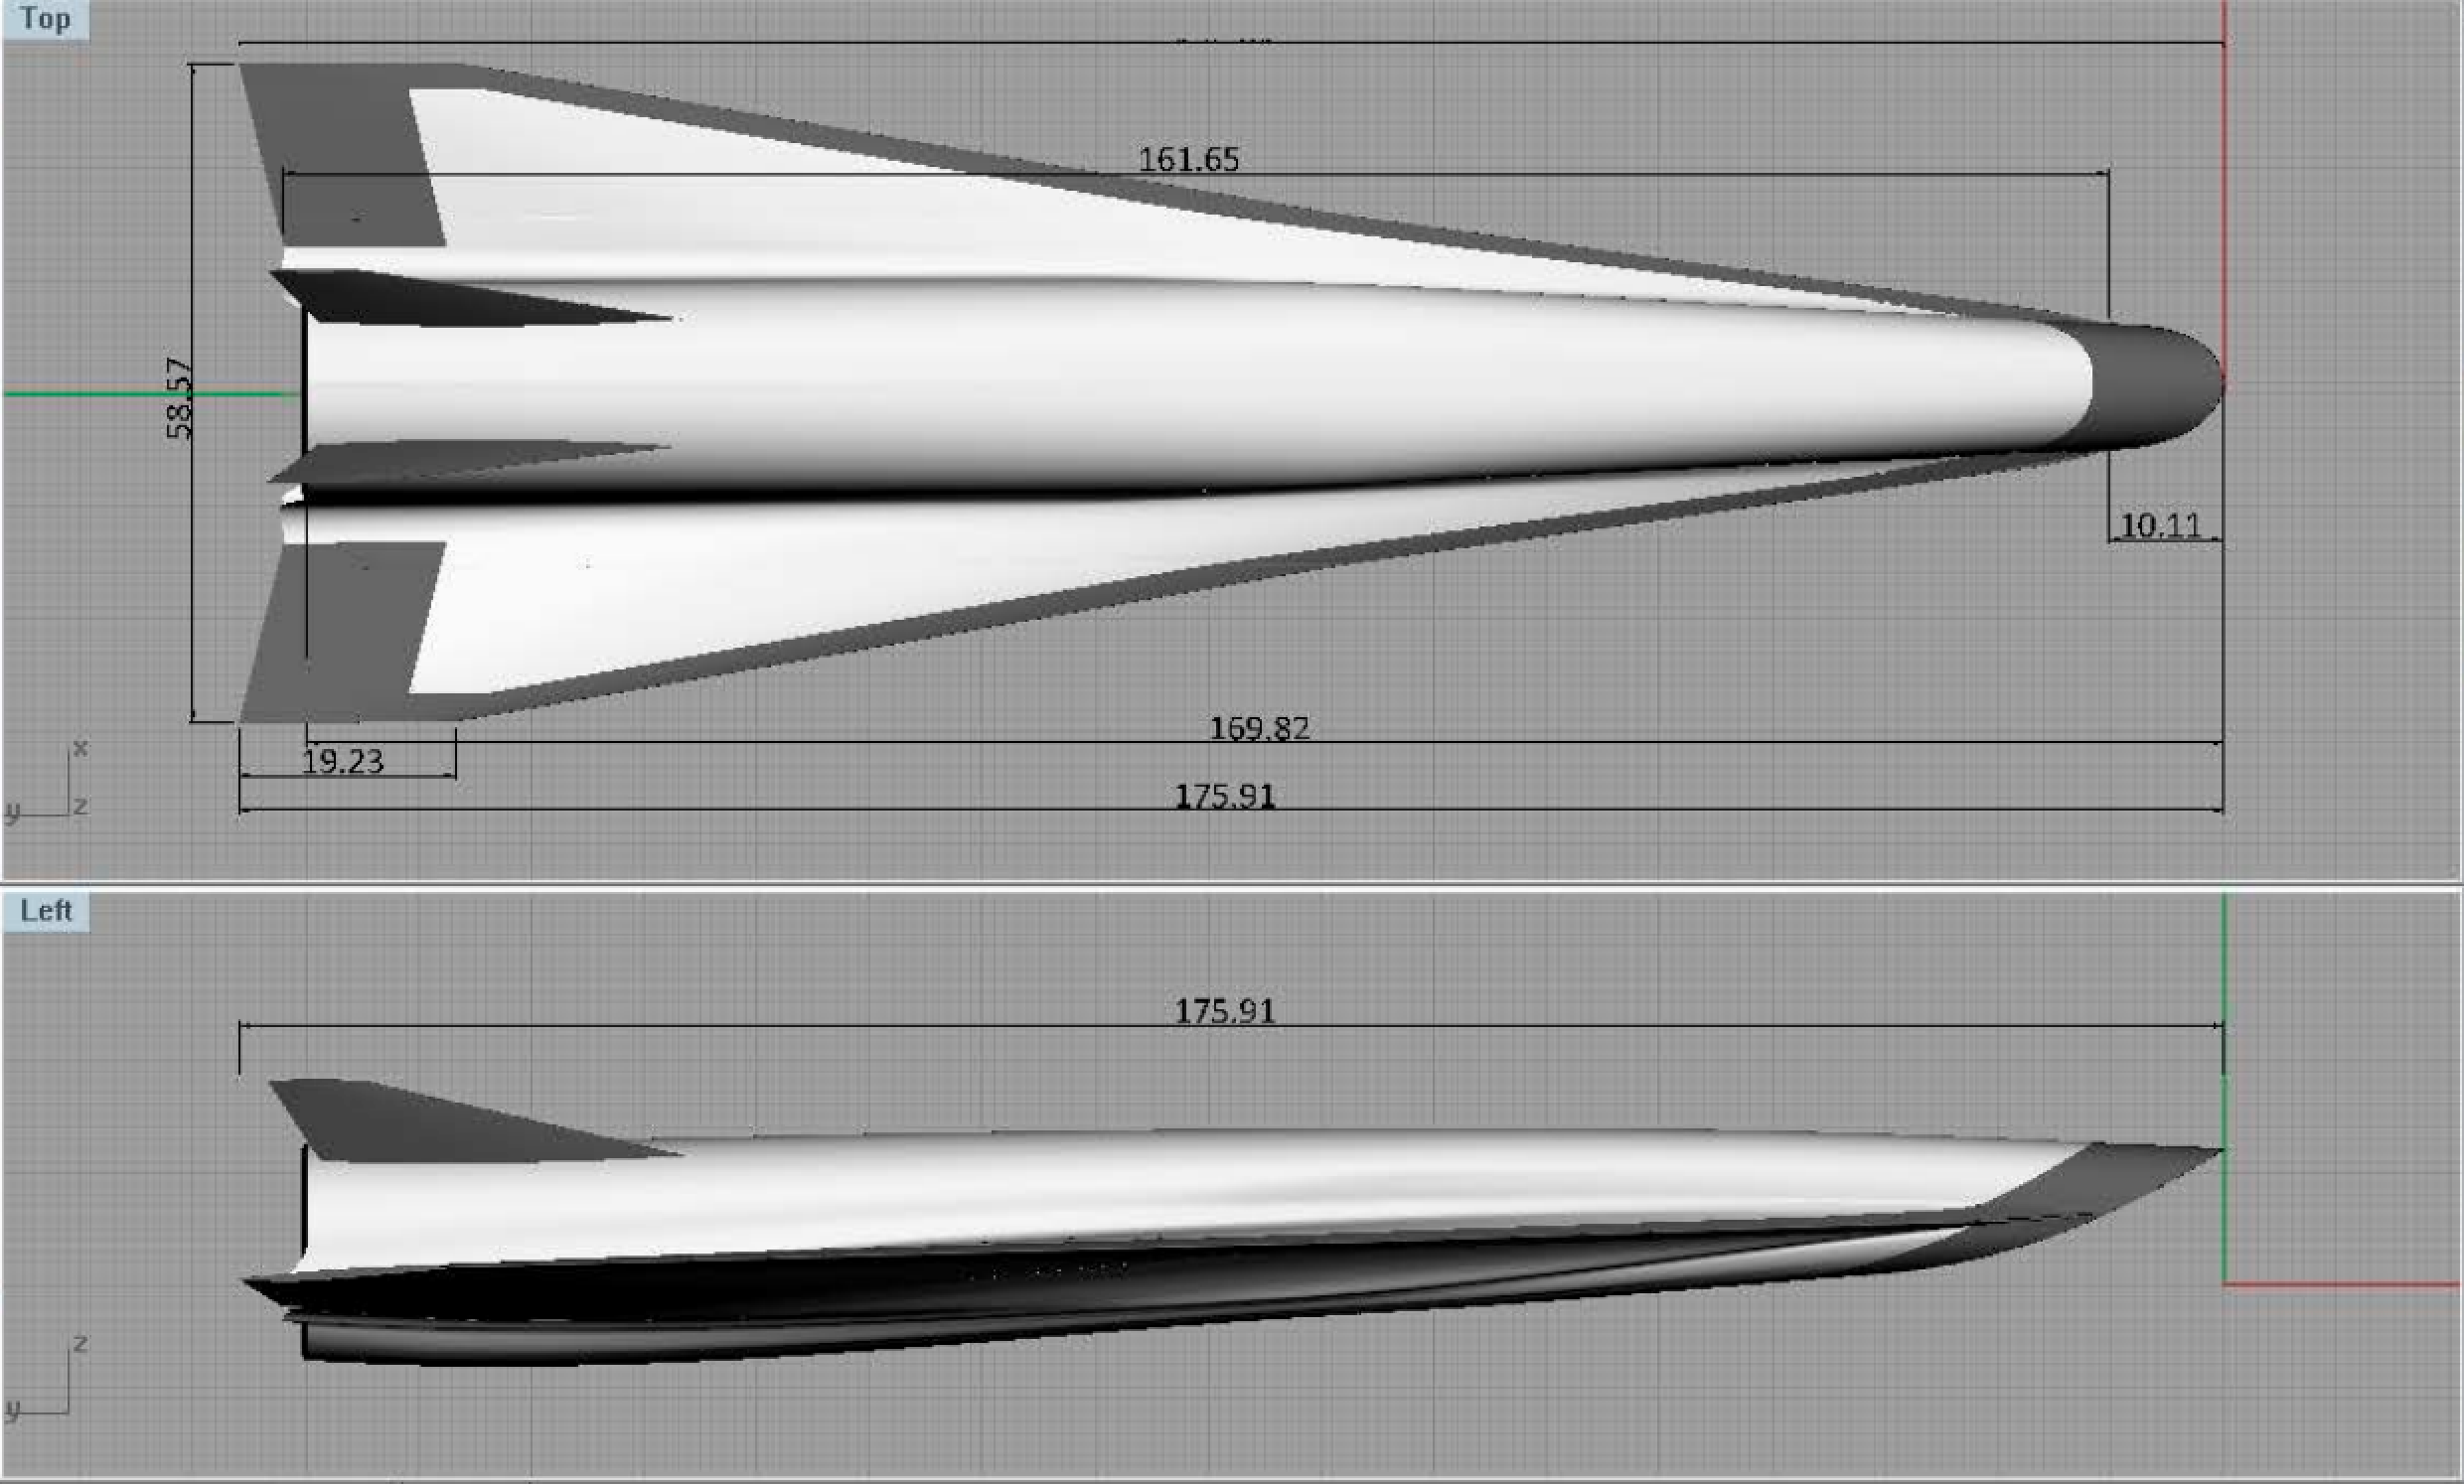
\includegraphics[width=4.5in]{\figurepath/ghvmodelview.png}
      \vspace{-0.1in}
      \caption{AFRL Road Runner generic hypersonic vehicle\label{fig:ghv_clouds}}
    \end{center}
  \end{figure}

  Aerodynamic and engine data for this model are stored in look-up tables within the simulation package.
  The aerodynamic look-up tables take as inputs the flight Mach number, angle of attack, sideslip angle, and control surface deflections to calculate the total aerodynamic forces and moments acting on the vehicle.
  The aerodynamic data for the GHV were calculated using the Supersonic/Hypersonic Arbitrary Body Program (S/HABP) code.
  The engine look-up tables take as inputs the flight Mach number, angle of attack, dynamic pressure, and equivalence ratio (throttle).
  The engine data were calculated using the Ramjet Performance Analysis (RJPA) code developed at the Applied Physics Laboratory at Johns Hopkins University.
  Some relevant vehicle properties are in Table~\ref{tab:vehicle_properties}.

  \begin{table}[H]
    \centering
    \caption{Vehicle properties}
    \begin{tabular}{llr}
      \toprule
      Parameter & Unit & Value \\ \midrule
      Gross weight & [lbm] & $1220.3$ \\
      Vehicle length & [in] & $175.9$ \\
      Span & [in] & $58.6$ \\
      Planform & [ft$^{2}$] & $42.178$ \\
      \bottomrule
    \end{tabular}\label{tab:vehicle_properties}
  \end{table}

  The equations of motion describing the GHV can be represented in state-space form as
  \begin{equation*}
    \dot{X}=f({X},U)
  \end{equation*}
  with state vector
  \begin{equation}
    \label{eqn:fullstatevector_x}
    X=\left[
    \begin{array}{cccccccccccc}
      V_{T} &  \alpha & q &\theta & h & \beta &p & r & \phi &\psi &\lambda & \tau
    \end{array}\right]^{\top}
  \end{equation}
  where $V_{T}$ is the total velocity, $\alpha$ and $\beta$ are the angle of attack and sideslip, $\phi$, $\theta$, and $\psi$ are the roll, pitch, and yaw angles, $p$, $q$, and $r$ are the absolute angular velocity components, and $\lambda$, $\tau$, and $h$ are the latitude, longitude, and altitude, of the GHV, respectively.
  The input vector is given by
  \begin{equation}
    \label{eqn:fullcontrolvector}
    U=\left[
    \begin{array}{cccc}
      \delta_{\text{th}} & \delta_{\text{elv}} & \delta_{\text{ail}} & \delta_{\text{rud}}
    \end{array}\right]^{\top}
  \end{equation}
  where $\delta_{\text{th}}$, $\delta_{\text{elv}}$, $\delta_{\text{ail}}$, and $\delta_{\text{rud}}$ are the throttle, elevator, aileron, and throttle inputs, respectively.

  The entries of the state vector are arranged so as to facilitate separation of the lateral and longitudinal equations of motion during control design.
  The deflection of the elevons is accomplished through static mixing, combining differential and collective deflections from the aileron and elevator commands, respectively, while both rudders are actuated together using the single rudder input.
  The control vector $U_{5}$ contains the deflections of the right and left elevons ($\delta_{r,\text{elv}}$, $\delta_{l,\text{elv}}$), rudders ($\delta_{r,\text{rud}}$, $\delta_{l,\text{rud}}$), and throttle as
  \begin{equation*}
    U_{5}=
    \left[
    \begin{array}{ccccc}
      \delta_{\text{th}} & \delta_{r,\text{elv}} & \delta_{l,\text{elv}} & \delta_{r,\text{rud}}  & \delta_{l,\text{rud}}
    \end{array}\right]^{\top}
  \end{equation*}
  The control allocation matrix $M$ is the matrix which defines the following transformation between control vectors $U_{5}$ and $U$ as
  \begin{equation*}
    U=MU_{5}
  \end{equation*}
  where control allocation matrix is
  \begin{equation*}
    M=
    \left[
    \begin{array}{ccccc}
      1 & 0 & 0 & 0 & 0 \\
      0 & 1/2 & 1/2 & 0 & 0 \\
      0 & 1/2 & -1/2 & 0 & 0 \\
      0 & 0 & 0 & 1/2 & 1/2 \\
    \end{array}\right]
  \end{equation*}

  \subsection{Actuator and Sensor Models}

  The propulsion system is modeled as a first order system with a cutoff frequency of 10 rad/s to capture fuel system delivery limits.
  Second order actuators with rate and deflection limits were included in the simulation model on all four of the aerodynamic control surfaces.
  The transfer function for the control surface actuators is
  \begin{equation*}
    G_{\text{cs}}(s)=\frac{{\omega_{n}}^{2}}{s^{2}+2\zeta\omega_{n}s+{\omega_{n}}^{2}}
  \end{equation*}
  and the block diagram for the control surfaces as implemented is shown in Figure~\ref{fig:actuator_block}, where the signal $u_{\text{cmd}}$ is generated by the controller, and due to the actuator dynamics the actual control surface deflection is given by $u_{\text{sat}}$.

  \begin{figure}[H]
    \fontsize{12pt}{12pt}\selectfont
    \begin{center}
      \begin{tikzpicture}[auto, scale=0.9, every node/.style={transform shape}, node distance=1.5cm, >=latex']
        \node[input](input1){};
        \node[satnode,draw,fill=white, minimum height=1.0cm, minimum width=1.0cm, right of=input1, node distance=1.5cm, label=below:{\shortstack{deflection \\ saturation}}] (block1){};
        \node[whitesum, right of=block1,node distance=1.8cm](sum1){$+$};
        \node[squareblock, right of=sum1,node distance=1.8cm] (block2){$\omega_{n}^{2}$};
        \node[whitesum, right of=block2, node distance=1.8cm](sum2){$+$};
        \node[squareblock, right of=sum2,node distance=1.8cm] (block3){$\frac{1}{s}$};
        \node[satnode,draw,fill=white, minimum height=1.0cm, minimum width=1.0cm, right of=block3, node distance=2.5cm, label=below:{\shortstack{rate \\ saturation}}] (block4){};
        \node[squareblock, right of=block4,node distance=2.0cm] (block5){$\frac{1}{s}$};
        \node[satnode,draw,fill=white, minimum height=1.0cm, minimum width=1.0cm, right of=block5, node distance=2.0cm, label=below:{\shortstack{deflection \\ saturation}}] (block6){};
        \node[output, right of=block6,node distance=1.5cm] (output1) {};
        \node[squareblock, below of=block3,node distance=2.0cm] (block7){$2\zeta\omega_{n}$};
        \node[tee,below of=block7,node distance=1.5cm] (tee1){};
        %Draw lines
        \draw[->](input1) -- node[near start]{$u_{\text{cmd}}$} (block1);
        \draw[->](block1) -- node[near end]{$+$} (sum1);
        \draw[->](sum1) -- (block2);
        \draw[->](block2) -- node[near end]{$+$} (sum2);
        \draw[->](sum2) -- node{$\ddot{u}$} (block3);
        \draw[->](block3) -- node[pos=0.4,name=u]{$\dot{u}$} (block4);
        \draw[->](block4) -- (block5);
        \draw[->](block5) -- node[pos=0.4,name=y]{$u$} (block6);
        \draw[->](block6) -- node[near end]{$u_{\text{sat}}$} (output1);
        \draw[->](u) |- (block7);
        \draw[->](block7) -| node[pos=0.95]{$-$} (sum2);
        \draw[-](y) |- (tee1);
        \draw[->](tee1) -| node[pos=0.95]{$-$} (sum1);
      \end{tikzpicture}
      \caption{Second order actuator block diagram\label{fig:actuator_block}}
    \end{center}
  \end{figure}

  The relevant values used in the second order aerodynamic control surface actuators are listed in Table~\ref{tab:actuator}.
  \begin{table}[H]
    \centering
    \caption{Second order aerodynamic control surface actuator parameters\label{tab:actuator}}
    \begin{tabular}{llc}
      \toprule
      Parameter & Unit & Value \\ \midrule
      Elevon deflection limit & [deg] & $-30$ to $30$ \\
      Rudder deflection limit & [deg] & $-30$ to $30$ \\
      Elevon rate limit & [deg/s] & $-100$ to $100$ \\
      Rudder rate limit & [deg/s] & $-100 $ to $100$ \\
      Damping ratio $\zeta$ & & $0.7$ \\
      Natural frequency $\omega_{n}$ & [rad/s] & $150$ \\
      \bottomrule
    \end{tabular}
  \end{table}
  First order low-pass filters were placed at the sensor outputs in order to reduce sensor noise being fed back to the controller.
  The velocity filter has a cutoff frequency of 20 rad/s, while the incidence, angular rate, and Euler angle sensor filters all have a cutoff frequency of 150 rad/s.
  These filters are implemented to model the effect of a navigation filter in the control loop.

  \subsection{Implementation}

  The GHV simulation block diagram is in Figure~\ref{fig:ghvcontrolblock}.
  The controller was implemented in discrete time and operated at 100 Hz with a zero-order hold on the control signal output.
  The output sensors are operated at 600 Hz, white noise was injected into the sensor signals, and an input time delay was used.

  \begin{figure}[H]
    \begin{center}
      \begin{tikzpicture}[auto, scale=0.8, every node/.style={transform shape}, node distance=1.0cm, >=latex']
        \node[squareblock, minimum height=1cm, minimum width=2cm, label=below:{100 Hz}] (block1){Controller};
        \node[input,left=of block1.170, node distance=2.0cm] (j1) {};
        \node[left of=j1, node distance=0.5cm] (input1) {};
        \node[input,left=of block1.190, node distance=1.0cm] (input2) {};
        \node[squareblock, minimum width=1cm, right of=block1, node distance=2.5cm] (block2) {$\tau_{\text{delay}}$};
        \node[squareblock, minimum height=1cm, minimum width=1.0cm, label=below:{\shortstack[c]{Actuator\\Dynamics}}, right of=block2,node distance=2.5cm, inner sep= 1mm] (block3) {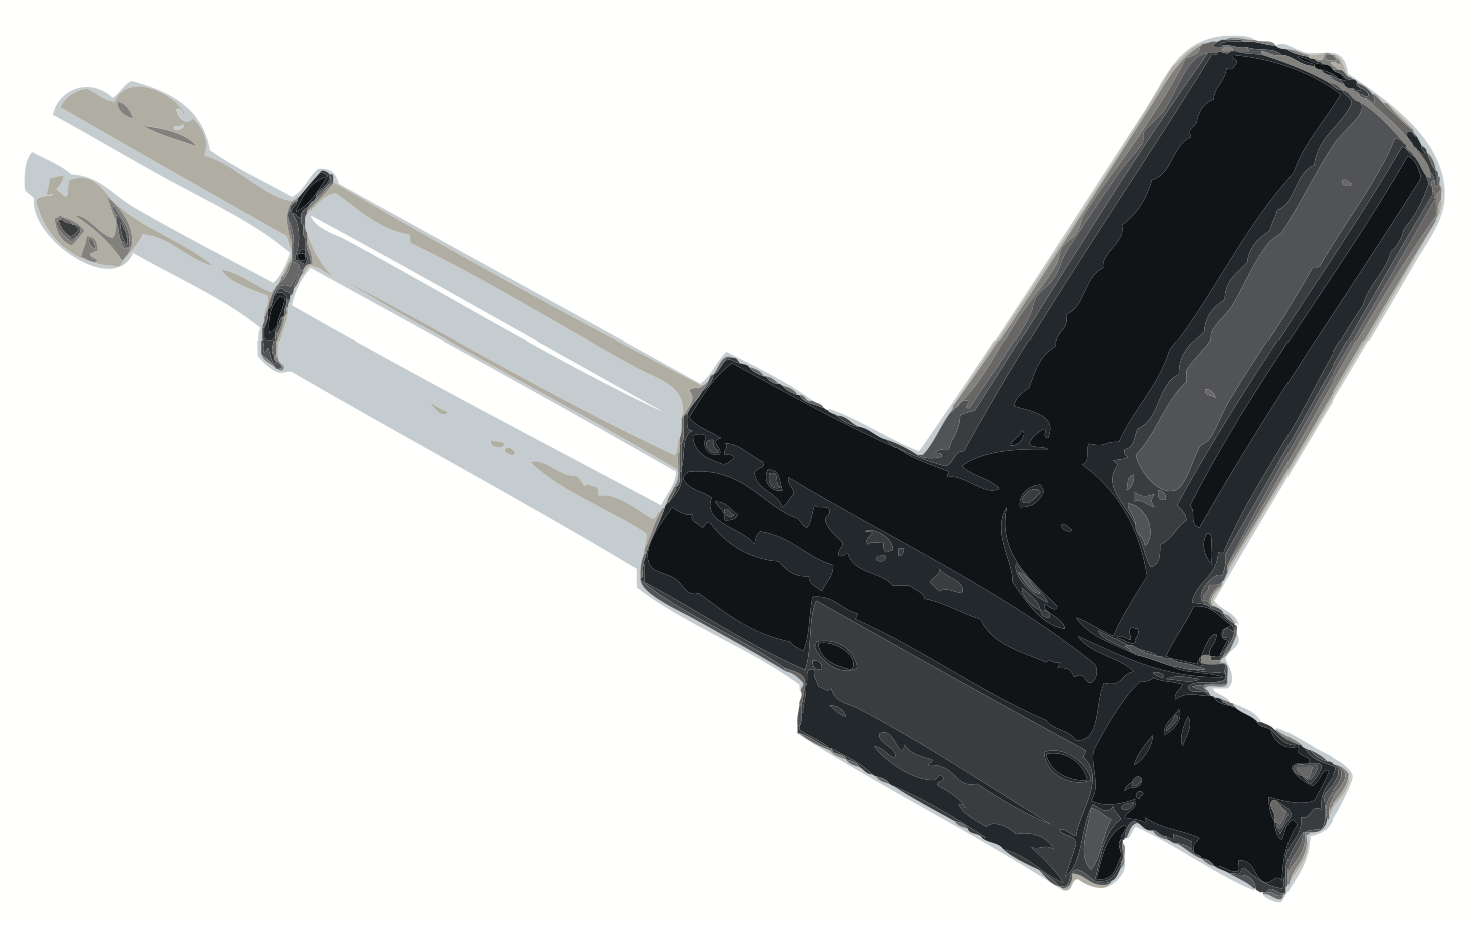
\includegraphics[width=1.6cm]{\figurepath/actuator_image.png}};
        \node [right of=block3,draw=black, anchor=west,node distance=2.0cm, minimum width=2cm, label=below:{Plant}, inner sep= 0mm] (block4) {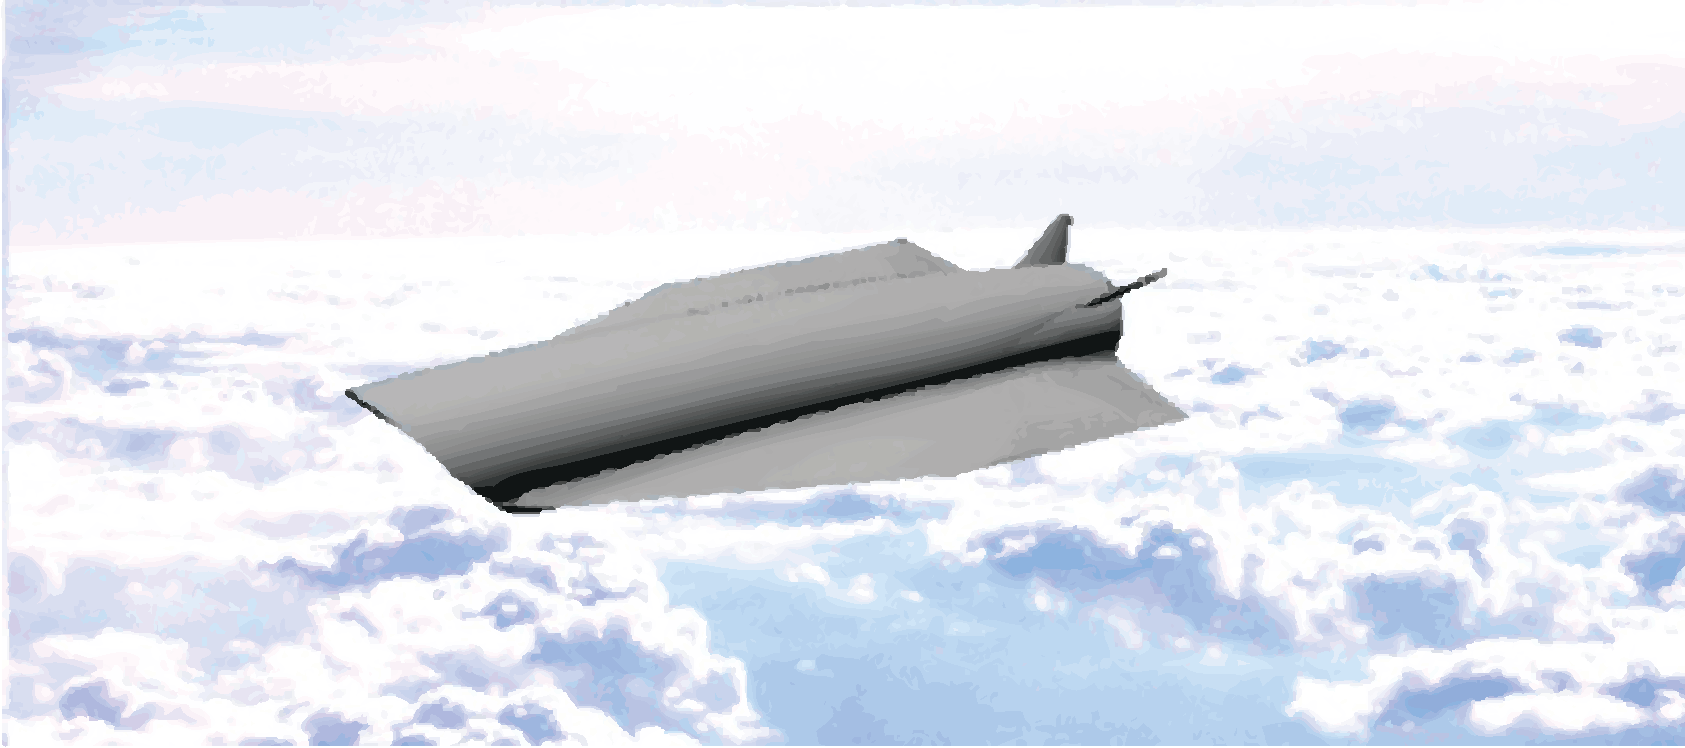
\includegraphics[width=4cm]{\figurepath/ghvclouds.pdf}};
        \node[whitesum, right of=block4,node distance=3.0cm] (sum1) {$+$};
        \node[input, above of=sum1,node distance=1.2cm](input3){};
        \node[squareblock, minimum width=1cm, right of=sum1, node distance=2.0cm] (block5) {ZOH};
        \node[squareblock, minimum width=1cm, right of=block5, node distance=2.0cm] (block6) {Filter};
        \node[output, right of=block6,node distance=2.0cm] (output1) {};
        \node[tee, below of=block3,node distance=1.8cm](tee1){};
        %Draw lines
        \draw[-](input1) -- node[near start]{$z_{\text{cmd}}$} (j1);
        \draw[->](j1) -- (block1.170);
        \draw[->](input2) -- (block1.190);
        \draw[->](block1) -- (block2);
        \draw[->](block2) -- (block3);
        \draw[->](block3) -- (block4);
        \draw[->](block4) -- (sum1);
        \draw[->](input3) -- (sum1);
        \draw[->](sum1) -- (block5);
        \draw[->](block5) -- node[name=n,pos=0.5]{}(block6);
        \draw[->](block6) -- node[name=y,pos=0.7]{} node[near end]{$x$}(output1);
        \draw[-](y) |- node[pos=0.9] {} (tee1);
        \draw[-](tee1) -| (input2);
        %Model box
        \begin{pgfonlayer}{background}
          \path (block5 |- block5)+(-1.0,0.7) node (c) {};
          \path (block6 -| block6)+(1.0,-0.7) node (d) {};
          \path[fill=gray!20, draw, dashed] (c) rectangle (d);
        \end{pgfonlayer}
        \node [above of=sum1, node distance = 1.5cm] {noise};
        \node[below of=n,node distance=1.2cm]{600 Hz};
      \end{tikzpicture}
      \caption{GHV flight control simulation block diagram\label{fig:ghvcontrolblock}}
    \end{center}
  \end{figure}

  \section{Open-Loop Analysis}

  The open-loop behavior of the GHV was analyzed about a nominal flight condition of $M=6$, $h=80,000$ ft, corresponding to a dynamic pressure of 1474 psf.
  The geographical coordinates and heading of the GHV are insignificant in the equations of motion for the purposes of inner-loop control law development\cite{journal:billimoriaschmidt1995}, and these state variables are dropped from the state vector in Eq.\ \eqref{eqn:fullstatevector_x} for trim, linearization, and control.

  \begin{equation}
    \label{eqn:truncstatevector_x}
    X=\left[
    \begin{array}{ccccccccc}
      V_{T} &  \alpha & q &\theta & h & \beta &p & r & \phi
    \end{array}\right]^{\top}
  \end{equation}
  The state $X\in\mathbb{R}^{n}$ from this point forward is used to mean the truncated state in Eq. (\ref{eqn:truncstatevector_x}), and the dynamics of the system that uses the truncated state are described by
  \begin{equation}
    \label{eqn:xdotfxu}
    \dot{X}=f({X},U)
  \end{equation}
  The trimmed state $X_{\text{eq}}$, and input $U_{\text{eq}}$ satisfy
  \begin{equation}
    \label{eqn:eqptdef}
    \dot{X}_{\text{eq}}=f({X}_{\text{eq}},U_{\text{eq}})=0
  \end{equation}
  The equilibrium state $X_{\text{eq}}$ is found for the nominal steady, level cruise condition, and the equations of motion in Eq. (\ref{eqn:xdotfxu}) describing the GHV are linearized about this trim state.
  Defining $x$ and $u$ to be state and input perturbations about equilibrium we have
  \begin{align*}
    X&=X_{\text{eq}}+x \\
    U&=U_{\text{eq}}+u
  \end{align*}
  The linearization results in the state-space system given below
  \begin{equation}
    \label{eqn:linss}
    \dot{x}=Ax+Bu
  \end{equation}

  Using this linear system, the open-loop dynamic modes of the GHV during the nominal steady, level cruise condition are analyzed through a sensitivity analysis.

  \subsection{Sensitivity Analysis}

  The methods of reference [\citen{manual.durham.2002}] were used to calculate the sensitivity matrix for the linear system given in Eq. (\ref{eqn:linss}).
  The sensitivity analysis indicated the presence of two longitudinal and three lateral flight modes as shown in Figure~\ref{fig:poleplot}.

  \begin{figure}[H]
    \centering
    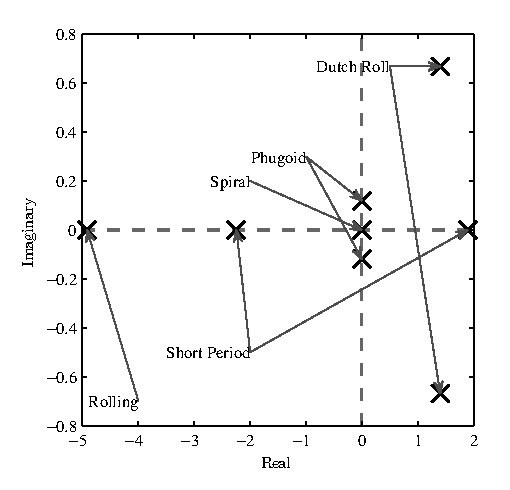
\includegraphics[width=3.0in]{\figurepath/openlooppoles_v2.eps}
    \caption{Open-loop poles of $A$ for $M=6$, $h=80,000$ ft steady, level cruise\label{fig:poleplot}}
  \end{figure}

  The sensitivity analysis aims to determine which entries in a given eigenvector are small when the units of each state variable are not the same.
  This method examines slight changes in the initial condition of each state separately, in order to determine whether this change will influence some modes more strongly than others.
  This analysis will provide knowledge of what modes the GHV exhibits, which states are dominant in each of these modes, and the stability of the modes.
  This knowledge will facilitate the control design process.
  Comparing the magnitude of the entries in the sensitivity matrix for the GHV, each of the modes was separated by at least one order of magnitude difference, indicating a strong decoupling of the flight modes.

  The GHV has a highly unstable irregular short period mode, dominated by $\alpha$ and $q$, and an unstable dutch roll mode.
  The phugoid mode is neutrally stable, and the rolling mode is stable.
  The velocity mode is given by a pole at the origin, and is omitted from Figure~\ref{fig:poleplot}.
  This analysis allowed the velocity, longitudinal, and lateral-directional subsystems to be decoupled, and each of these three plant subsystems to be represented as
  \begin{equation}
    \label{eqn:plantxp}
    \dot{x}_{p}=A_{p}x_{p}+B_{p}u
  \end{equation}
  where $x_{p}\in\mathbb{R}^{n_{p}}$, $A_{p}\in\mathbb{R}^{n_{p}\times n_{p}}$, $B_{p}\in\mathbb{R}^{n_{p}\times m}$ and $u\in\mathbb{R}^{m}$.
  Note that these sizes will differ for each of the subsystems.

  \subsection{Representation of Uncertainties}\label{sec:repofuncertainties}

  It can be shown that the parametric uncertainties considered in this work and described above manifest themselves in the linear system given in Equation (\ref{eqn:plantxp}) as
  \begin{equation}
    \label{eqn:xdotpunc}
    \dot{x}_{p}=A_{p\lambda}x_{p}+B_{p\lambda}u
  \end{equation}
  where
  \begin{equation}
    \label{eqn:linearuncertainties}
    A_{p\lambda}=A_{p}+B_{p}\Lambda{W_{p}}^{\top}
    \hspace{0.5in}
    B_{p\lambda}=B_{p}\Lambda
  \end{equation}
  $\Lambda\in\mathbb{R}^{m\times m}$ and $W_{p}\in\mathbb{R}^{n_{p}\times m}$.
  These uncertainties are called ``matched'' uncertainties, as they enter the system dynamics through the control channels\ \cite{book.lavretskywise.2013}.
  The adaptive controller that is designed in Section~\ref{sec:adaptivedesign} is carried out so as to accommodate such uncertainties.
  Other unmatched uncertainties, such as sensor bias/noise are introduced as well, and the control design must be sufficiently robust to these, as they are not accommodated for explicitly in the synthesis of the controller.

  \section{Baseline Control Design}\label{sec:baselinedesign}

  This section outlines the basic architecture used for the inner loop flight controller.
  The baseline flight controller will be used to stabilize the GHV during flight, and track reference commands.
  The modal analysis showed a strong separation between velocity, longitudinal, and lateral-directional dynamics of the GHV.\
  This separation allows these dynamics to be considered independently for control design, allowing several lower order controllers to be designed, as opposed to a single higher order one.
  In addition, due to the timescale separation between the short period and phugoid modes, only the fast states, $\alpha$ and $q$, are used for longitudinal feedback control.
  The following table summarizes the order of each of the three subsystems for which a full-state feedback LQR-PI controller will be designed.

  \begin{table}[H]
    \centering
    \caption{Plant Subsystem Order}
    \fontsize{10pt}{10pt}\selectfont
    \begin{tabular}{lcc}
      \toprule
      Subsystem & Order $(n_{p})$ & Feedback States \\
      \midrule
      Velocity & 1 & $V_{T}$ \\
      Longitudinal & 2 & $\alpha$, $q$ \\
      Lateral & 4 & $\beta$, $p$, $r$, $\phi$ \\
      \bottomrule
    \end{tabular}
  \end{table}

  The velocity and longitudinal subsystems are both single input systems.
  The throttle input $\delta_{\text{th}}$ controls only the velocity $V_{T}$, and the elevator input $\delta_{\text{elv}}$ controls the longitudinal states.
  The lateral subsystem is multi-input, with the aileron $\delta_{\text{ail}}$ and tail $\delta_{\text{rud}}$ as control inputs.

  Each linear subsystem is expressed using the state-space representation with the regulated output $z$ as follows
  \begin{equation}
    \label{eqn:plantss_xp}
    \begin{split}
      \dot{x}_{p}&=A_{p}x_{p}+B_{p}u \\
      z&=C_{zp}x_{p} \\
    \end{split}
  \end{equation}
  where $C_{pz}\in\mathbb{R}^{n_{e}\times n_{p}}$, and $z\in\mathbb{R}^{n_{e}}$.
  Note again that these sizes will differ for each of the subsystems.
  For each of the three subsystems described by Eq. (\ref{eqn:plantss_xp}) an LQR-PI baseline controller is designed assuming the plant parameters are fully known.
  The LQR-PI control architecture is represented by the following block diagram, where $d_{\text{in}}$ is an input load disturbance, $d_{\text{out}}$ is an output load disturbance or sensor bias, and $n$ is sensor noise.

  \begin{figure}[H]
    \begin{center}
      \fontsize{12pt}{12pt}\selectfont
      \begin{tikzpicture}[auto, scale=0.8, every node/.style={transform shape}, node distance=1.0cm, >=latex']
        \node[squareblock, minimum height=2cm, minimum width=2cm, label=above:{Controller}] (block1){$K(s)$};
        \node[left=of block1.150, node distance=5.0cm] (j1) {};
        \node[left of=j1, node distance=1.9cm] (input1) {};
        \node[whitesum,left=of block1.200, node distance=1.5cm] (sum1) {};
        \node[input, left of=sum1, node distance=1.5cm](input2){};
        \node[whitesum, right of=block1, node distance=2.5cm] (sum2) {};
        \node[input, above of=sum2,node distance=1.5cm](input3){};
        \node[squareblock, minimum height=2cm, minimum width=2cm, right of=sum2, label=above:{Plant},node distance=2.5cm] (block2) {$G(s)$};
        \node[whitesum, right of=block2,node distance=2.5cm] (sum3) {};
        \node[input, above of=sum3,node distance=1.5cm](input4){};
        \node[output, right of=sum3,node distance=2.5cm] (output1) {};
        \draw[->](sum3) --  node[name=yi,pos=0.4]{$y_{i}$}(output1);
        \node[whitesum, below of=yi,node distance=2.5cm] (sum4) {};
        \node[input, right of=sum4,node distance=1.5cm](input5){};
        \draw[->](input1) -- node[near start]{$z_{\text{cmd}}$} (block1.150);
        \draw[->](input2) -- node[near start]{$r$} node[pos=0.9] {$+$} (sum1);
        \draw[->](sum1) -- node{$e$} (block1.200);
        \draw[->](block1) -- node{$u_{o}$} node[pos=0.9]{$+$} (sum2);
        \draw[->](input3) -- node[near start]{$d_{\text{in}}$} node[pos=0.9] {$+$} (sum2);
        \draw[->](sum2) -- node{$u_{i}$} (block2);
        \draw[->](block2) -- node{$y_{o}$} node[pos=0.95] {$+$} (sum3);
        \draw[->](input4) -- node[near start]{$d_{\text{out}}$} node[pos=0.9] {$+$} (sum3);
        \draw[->](yi) -- node[pos=0.9] {$+$} (sum4);
        \draw[->](input5) -- node[near start]{$n$} node[pos=0.9] {$-$} (sum4);
        \draw[->](sum4) -| node{$w$} node[pos=0.95] {$-$} (sum1);
      \end{tikzpicture}
      \caption{General MIMO feedback control block diagram\label{fig.lqrpiblock}}
    \end{center}
  \end{figure}

  The integral error states are added by differencing a collection of perturbation state variables of interest and the corresponding reference value $z_{\text{cmd}}$ as follows.
  \begin{equation}
    \label{eqn:integralerrorstate}
    \dot{x}_{e}=z_{\text{cmd}}-z
  \end{equation}
  Using the error description in Eq. (\ref{eqn:integralerrorstate}), the state vector $x_{p}$ from the plant in Eq. (\ref{eqn:plantss_xp}) is augmented to include the state error $x_{e}$ as a state variable as
  \begin{equation}
    \label{eqn.augssbig}
    \begin{bmatrix}
      \dot{x}_{p} \\
      \dot{x}_{e}
    \end{bmatrix} =
    \begin{bmatrix}
      A_{p} & 0 \\
      -C_{pz} & 0
    \end{bmatrix}
    \begin{bmatrix}
      x_{p} \\
      x_{e}
    \end{bmatrix}+
    \begin{bmatrix}
      B_{p} \\
      0
    \end{bmatrix}u+
    \begin{bmatrix}
      0 \\
      I
    \end{bmatrix}z_{\text{cmd}}
  \end{equation}
  Using $x=[\begin{array}{cc} x_{p}^{\top} & x_{e}^{\top} \end{array}]^{\top}$ the linear state-space representation in Eq. (\ref{eqn.augssbig}) can be expressed more compactly as
  \begin{equation}
    \label{eqn.augsssmall}
    \dot{x}=Ax+Bu+B_{\text{ref}}z_{\text{cmd}}
  \end{equation}
  where
  \begin{equation}
    A=
    \begin{bmatrix}
      A_{p} & 0 \\
      -C_{pz} & 0
    \end{bmatrix}
    \quad
    B=
    \begin{bmatrix}
      B_{p} \\
      0
    \end{bmatrix}
    \quad
    B_{\text{ref}}=
    \begin{bmatrix}
      0 \\
      I
    \end{bmatrix}
  \end{equation}
  and $A\in\mathbb{R}^{n\times n}$, $B\in\mathbb{R}^{n\times m}$, and $B_{\text{ref}}\in\mathbb{R}^{n\times n_{e}}$.
  The following baseline control law will is used for the integral-augmented plant
  \begin{equation}
    \label{eqn:lqrpilaw}
    u_{\text{bl}}=K_{\text{lqr}}^{\top}x
  \end{equation}
  where the gain $K_{\text{lqr}}$ is selected using LQR, and ensures $(A+BK_{\text{lqr}}^{\top})$ is a Hurwitz matrix.
  Such a baseline control law with integral action provides good frequency domain properties, and guarantees zero steady-state error through the addition of the integrator.

  The velocity and longitudinal subsystem were each augmented with an integrator to allow velocity and angle of attack commands to be tracked.
  The lateral controller was augmented with two integrators to command zero sideslip, and the desired roll angle.

  \subsection{Frequency Domain Analysis}

  While LQR optimization can simplify the control design process by reducing the selection of individual feedback gains to selection of cost function weights, there is still a lot of freedom left to tune the controller to achieve the desired performance.
  Each of the weighting matrices for the three baseline control subsystems were adjusted to return gains which would not be too large and demand an excessive rate or deflection from the actuators, but also that resulted in quick transient performance, command tracking with zero steady state error, and an acceptable level of robustness against noise and unmodeled dynamics.

  The LQR weighting matrix selection followed an iterative tuning process from reference [\citen{lavretskywisebook}].
  The objective is to set the control weighting matrix $R_{\text{lqr}}$ to an identity matrix, and use a diagonal state weighting matrix $Q_{\text{lqr}}$, initially with all entries zero except those corresponding to the integral error states.
  An algebraic Riccati equation is solved, yielding the optimal gain feedback matrix $K_{\text{lqr}}$.
  With this feedback gain matrix, the closed-loop system can then be analyzed by simulating the time response of the system, and by plotting frequency domain data.
  This process was repeated while adjusting only the integral error weights in $Q_{\text{lqr}}$ and the input weighting matrix $R_{\text{lqr}}$, to achieve the desired performance.
  The resulting LQR weighting matrices for the longitudinal control subsystem are shown below.

  \begin{equation*}
    Q_{\text{lqr,long}}=
    \text{diag}\bigr([
    \begin{array}{ccc}
      0 & 0 & 170
    \end{array}]\bigr)
    \hspace{0.5in}
    R_{\text{lqr,long}}=0.0001
  \end{equation*}
  The velocity and lateral subsystems had weighting matrices which were selected in the same way, with a nonzero weight placed on the lateral $Q_{\text{lqr}}$ matrix term corresponding to roll rate.
  This essentially added roll damping to the system.

  For the SISO plant sub-systems, the magnification of signals through the control loop depends only on the frequency of the signal, and so frequency domain data can be analyzed using Bode plots.
  The loop transfer function is found by breaking the control loop at either the input ($L_{u}$) or the output ($L_{y}$), and other transfer functions of interest are then calculated using the loop transfer function.
  In general, these two transfer functions will be different, but in the SISO case they are the same.

  In the case of MIMO systems, the magnification of signals through the control loop depends additionally on the direction of the input, and thus the singular values of the various transfer matrices were considered.
  By looking at the maximum and minimum singular values of these transfer matrices, much information can be determined about the relative stability of the control system.
  The six transfer matrices of interest, termed the ``gang-of-six'' in reference [\citen{book.astrommurray.2009}] are useful in examining the frequency domain properties of the system, and are plotted for each subsystem in the following figures.

  The maximum and minimum singular values of a transfer matrix $M(s)$ are denoted by $\overline{\sigma}(M)$ and $\underline{\sigma}(M)$, respectively.
  The singular value stability margins are defined using the return difference matrix $I+L_{u}$ and stability robustness matrix $I+L_{u}^{-1}$ as follows.
  First define
  \begin{equation*}
    \alpha_{\sigma}=\underline{\sigma}(I+L_{u})
    \hspace{0.5in}
    \beta_{\sigma}=\underline{\sigma}(I+L_{u}^{-1})
  \end{equation*}
  Calculate the phase margin and gain margin from the return difference matrix as
  \begin{equation}
    GM_{I+L}=\left[\frac{1}{1+\alpha_{\sigma}},\frac{1}{1-\alpha_{\sigma}}\right]\quad
    PM_{I+L}=\pm2\sin^{-1}\biggr(\frac{\alpha_{\sigma}}{2}\biggr)
  \end{equation}
  and from the stability robustness matrix as
  \begin{equation}
    GM_{I+L^{-1}}=\left[1-\beta_{\sigma},1+\beta_{\sigma}\right]\quad
    PM_{I+L^{-1}}=\pm2\sin^{-1}\biggr(\frac{\beta_{\sigma}}{2}\biggr)
  \end{equation}
  Taking the union of these two gain and phase margin expressions yield the following multivariable margins.
  \begin{equation}
    GM=GM_{I+L}\cup GM_{I+L^{-1}}\quad
    PM=PM_{I+L}\cup PM_{I+L^{-1}}
  \end{equation}
  These margins are more conservative than classical stability margins calculated for SISO systems.
  The delay margins are calculated as follows, where $\omega_{cg}$ is the loop gain crossover frequency, given by the frequency where $\overline{\sigma}(L_{u}(s))$ crosses 0 dB.
  \begin{equation*}
    \tau=\frac{PM}{\omega_{cg}}
  \end{equation*}
  Figures~\ref{fig:velbode}-\ref{fig:latrsingularval} show Bode plots for the velocity and longitudinal control subsystems for the LQR-PI controllers as designed for the plant at the nominal $M=6$, $h=80,000$ ft flight condition, and singular value plots for all three control subsystems.

  \begin{figure}[H]
    \begin{center}
      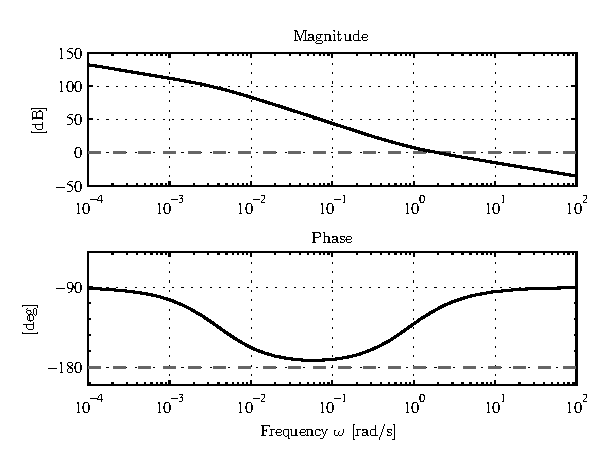
\includegraphics[width=3.2in]{\figurepath/results_vtotbode_v1.eps}
      \caption{Velocity loop transfer function Bode plot\label{fig:velbode}}
    \end{center}
  \end{figure}

  \begin{figure}[H]
    \begin{center}
      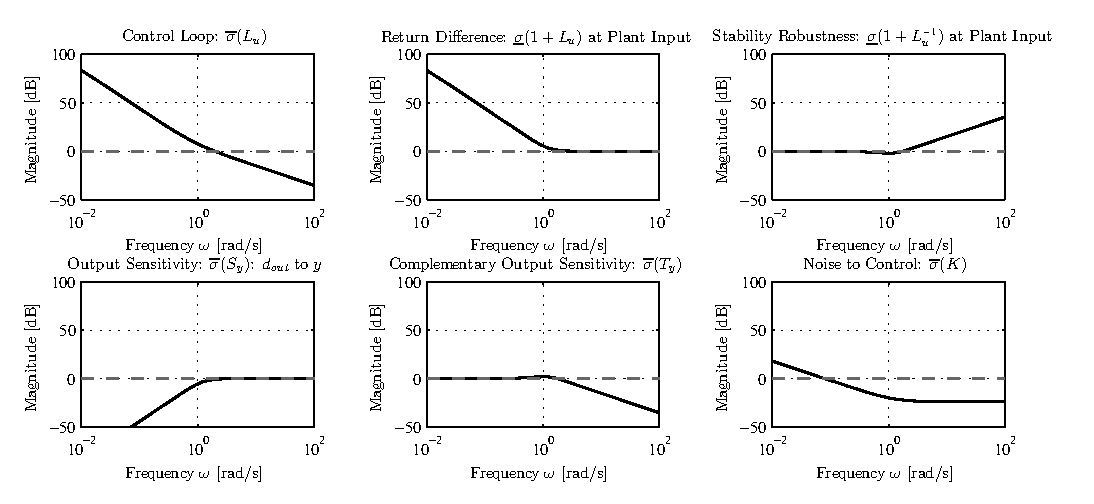
\includegraphics[width=5.0in]{\figurepath/results_vtotsigma_v1.eps}
       \caption{Velocity loop transfer function singular values}
    \end{center}
  \end{figure}

  \begin{figure}[H]
    \begin{center}
      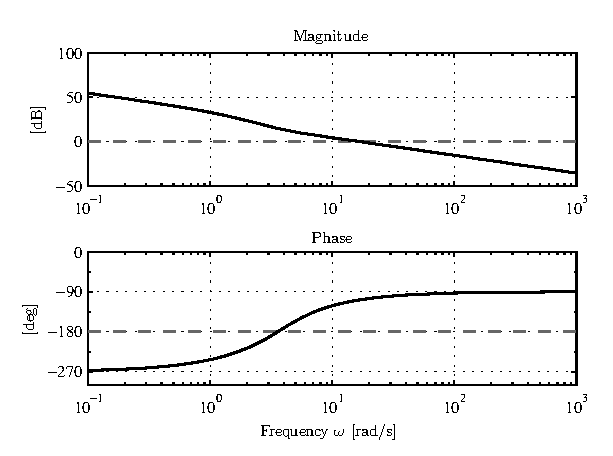
\includegraphics[width=3.2in]{\figurepath/results_longbode_v1.eps}
       \caption{Longitudinal loop transfer function Bode plot\label{fig:longbode}}
    \end{center}
  \end{figure}

  \begin{figure}[H]
    \begin{center}
      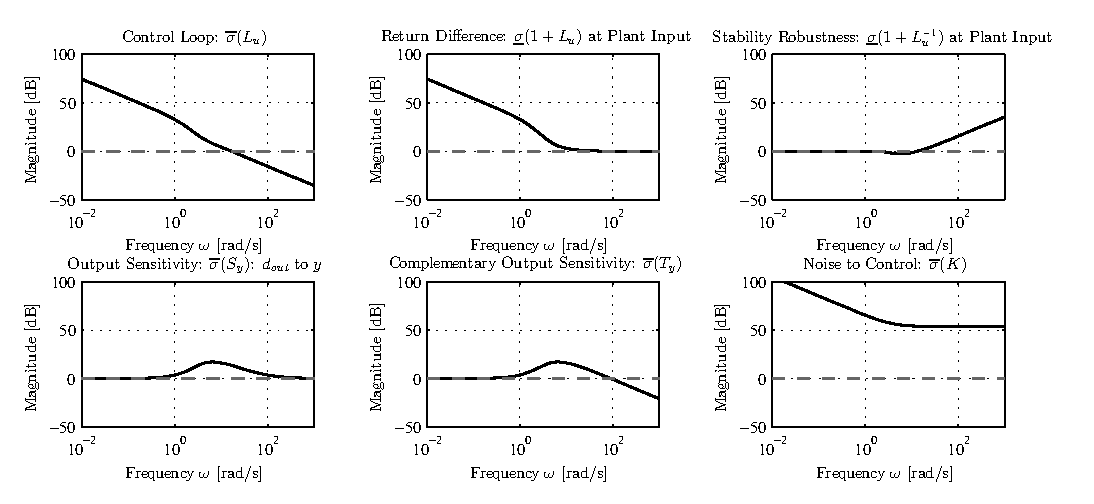
\includegraphics[width=5.0in]{\figurepath/results_longsigma_v1.eps}
       \caption{Longitudinal loop transfer function singular values\label{fig:longsigma}}
    \end{center}
  \end{figure}

  \begin{figure}[H]
    \begin{center}
      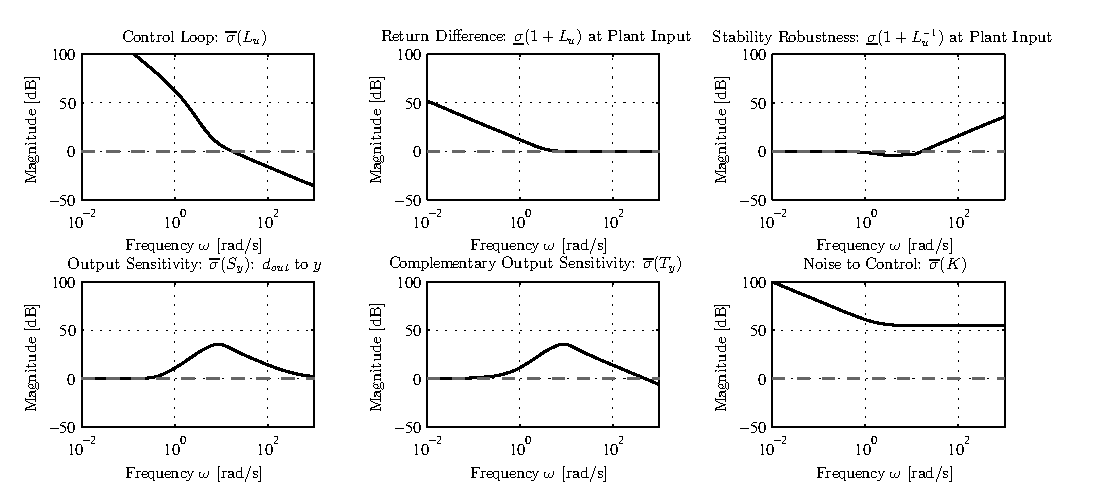
\includegraphics[width=5.0in]{\figurepath/results_latrsigma_v1.eps}
      \caption{Lateral loop transfer matrix singular values\label{fig:latrsingularval}}
    \end{center}
  \end{figure}

  \subsection{Inner Loop Controller Summary}

  For each of the three subsystems above, adjustment of the LQR weighting matrices was guided by time response plots, and Figures~\ref{fig:velbode}-\ref{fig:latrsingularval} above.
  As the feedback gains were increased, the GHV became more responsive, as indicated in time response data, but at the expense of reduced margins.
  As such, a balance was reached which gave both good time response performance and margins.
  The resulting crossover frequency of the loop transfer function for each subsystem is shown in Table~\ref{tab:crossover}.

  \begin{table}[H]
    \centering
    \caption{Loop transfer function crossover frequencies and margins\label{tab:crossover}}
    \small
    \begin{tabular}{lcccccc}
      \toprule
      Subsystem & Crossover [rad] & Crossover [Hz] & GM [dB] & PM [deg] & Delay margin [ms] \\
      \midrule
      Velocity & 1.95 & 0.31 & $\infty$ & 65.6 & 587 \\
      Longitudinal & 16.6 & 2.64 & -14.8 & 71.3 & 75.0 \\
      Lateral & 11.4--17.5 & 1.82--2.78 & $\bigr[
      \begin{array}{cc}
        -7.5 & 281.5
      \end{array}\bigr]$ & 43.9 & 43.8 \\
      \bottomrule
    \end{tabular}
  \end{table}

  It is desirable that the maximum singular value of the loop transfer function be sufficiently large at low frequencies for good command tracking, avoid an excessively large crossover frequency, and roll off at high frequency.
  The crossover frequency was selected so as to provide sufficiently large bandwidth tracking, while also maintaining separation from actuator bandwidth.

  \subsection{Gain Scheduling}

  Section~\ref{sec:baselinedesign} described the design of the baseline control gains using a linear model that was valid about a nominal trim point.
  For maneuvers which depart significantly from this nominal trim condition, the controller performance can deteriorate as the open-loop plant may be very different from the plant for which the controller was designed.
  For this reason, it was important to gain schedule the baseline controller over the entire flight envelope.

  The primary factor which affects how the open-loop plant behavior changes across the flight envelope is dynamic pressure, and this was used to schedule the feedback control gains.
  The dynamic pressure over which the GHV operates is from 800-2000 psf, and this range was broken into intervals of 100 psf for the schedule.
  The linearized dynamics of the GHV vary across dynamic pressure, changing the $A$ and $B$ matrices used in calculation of the feedback gain.
  In addition to using these matrices to determine the feedback gains at each scheduling point, the weighting matrices $Q_{\text{lqr}}$ and $R_{\text{lqr}}$ used in the cost function were also changed.
  A detailed frequency domain analysis could be performed for each scheduling point to select suitable weighting matrices.
  Instead, the nominal input weighting matrix $R_{\text{lqr}}$ was scheduled to be directly proportional to dynamic pressure, thereby penalizing large control inputs more when the dynamic pressure is high and such large control inputs are not necessary.

  The gain schedule was then created off-line, and produced an output containing the trim state and input at each operating point, the corresponding linear model, and the feedback gains.
  The nominal feedback gain is then changed by interpolating within the schedule using dynamic pressure.
  The scheduling interval of 100 psf was validated by evaluating controller performance at many points across the scheduling interval.

  \section{Adaptive Control Design}
  \label{sec:adaptivedesign}

  The baseline controller in the following section has been designed to have adequate margins, and should be robust to some reasonable variations in plant parameters.
  However, due to the magnitude of the uncertainties associated with hypersonic vehicles during flight, even a suitably robust baseline controller may not always be able to ensure stability.
  It is for this reason that adaptive augmentation was used.

  In the presence of parametric uncertainties, it is unknown how the GHV will respond to input commands during flight.
  However, under nominal circumstances the plant is known, and the baseline controller was designed to achieve an `ideal' response to a given input.
  A model-reference adaptive control (MRAC) structure was chosen as it will attempt to recover this nominal behavior by directly using the error between the ideal and actual response to drive parameter adaptation.
  The ideal response is provided by the reference model.
  This adaptive MRAC controller is designed to ensure good command tracking performance and stability in the presence of these uncertainties.\cite{narendra2005stable}
  In addition, the MRAC control architecture can be added without any modification to the baseline controller.
  This baseline-plus-adaptive control architecture is represented by the block diagram shown in Figure~\ref{fig.baseplusadaptiveblock}.

  \begin{figure}[H]
    \begin{center}
      \begin{tikzpicture}[auto, scale=0.85, every node/.style={transform shape}, node distance=1.0cm, >=latex']
        \node[squareblock, minimum height=1cm, minimum width=2cm] (block1){\shortstack[c]{Baseline\\Controller}};
        \node[squareblock, below of=block1, node distance=1.5cm, minimum height=1cm, minimum width=2cm] (block2){\shortstack[c]{Adaptive\\Controller}};
        \matrix[ampersand replacement=\&, row sep=0.5cm, left of=block1,node distance=1cm] (block1in) {%
        \node [coordinate] (b1inA) {};\\
        \node [coordinate] (b1inB) {};\\
        };
        \matrix[ampersand replacement=\&, row sep=0.5cm, left of=block2,node distance=1cm] (block2in) {%
        \node [coordinate] (b2inA) {};\\
        \node [coordinate] (b2inB) {};\\
        };
        \node [left of=b2inB, node distance=0.5cm] (2B) {};
        \node [below of=2B, node distance=0.12cm] (2B2) {};
        \node [left of=b2inA, node distance=1.0cm] (2A) {};
        \node [below of=2A, node distance=0.12cm] (2A2) {};
        \node[whitesum,right of=block1, node distance=2.5cm] (sum1) {};
        \node[squareblock, minimum height=1cm, minimum width=1.0cm, label=below:{\shortstack[c]{Actuator\\Dynamics}}, right of=sum1,node distance=2.5cm, inner sep= 1mm] (block3) {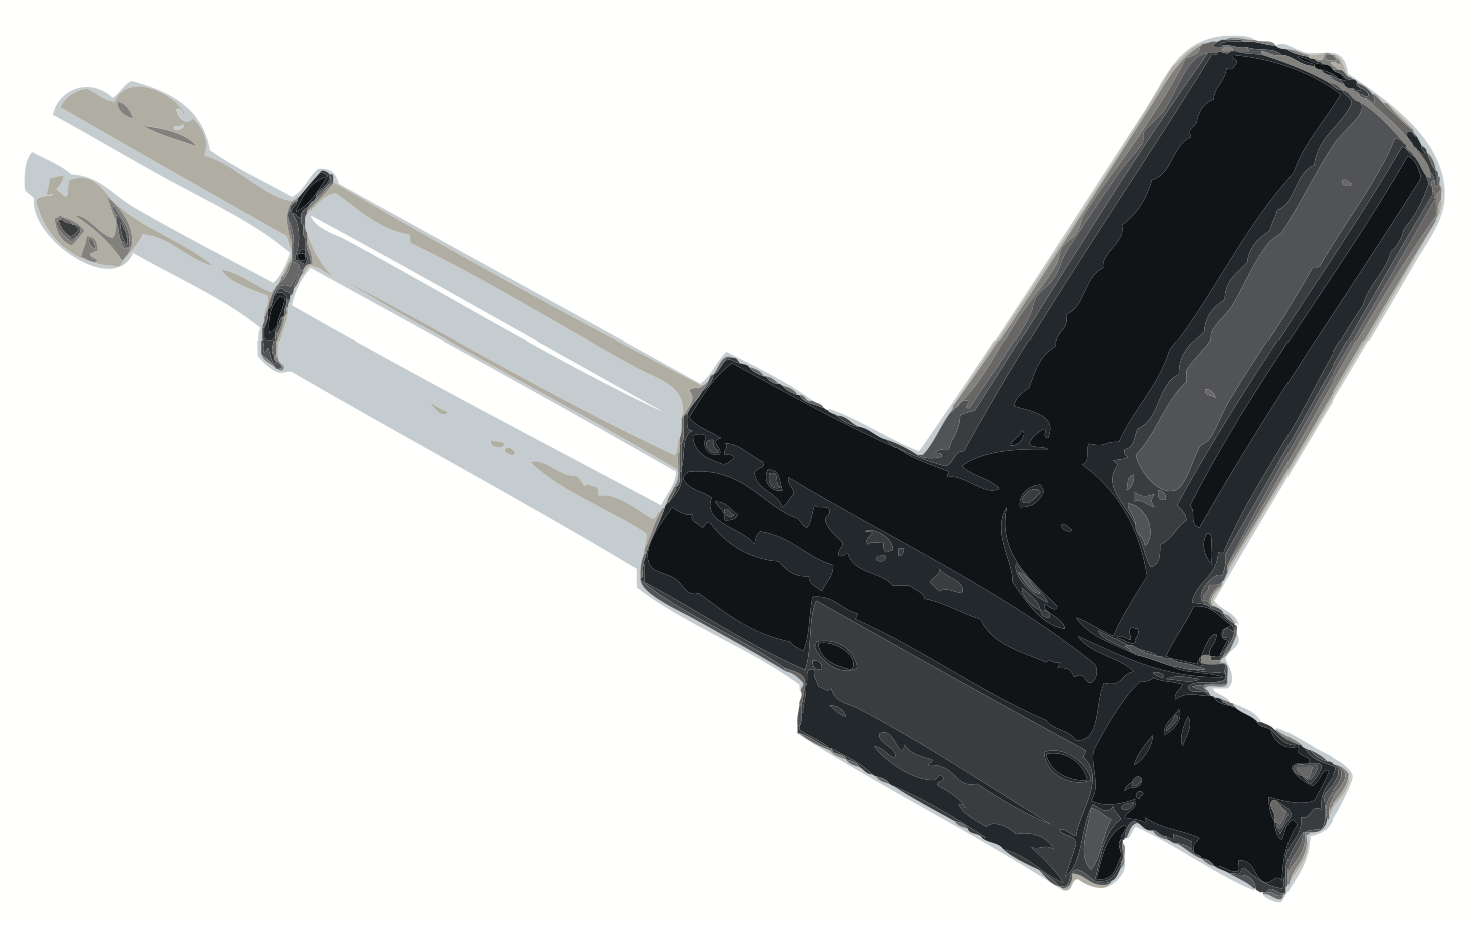
\includegraphics[width=1.6cm]{\figurepath/actuator_image.png}};
        \node [right of=block3,draw=black, anchor=west,node distance=2.0cm, minimum width=2cm, label=below:{Plant}, inner sep= 0mm] (block4) {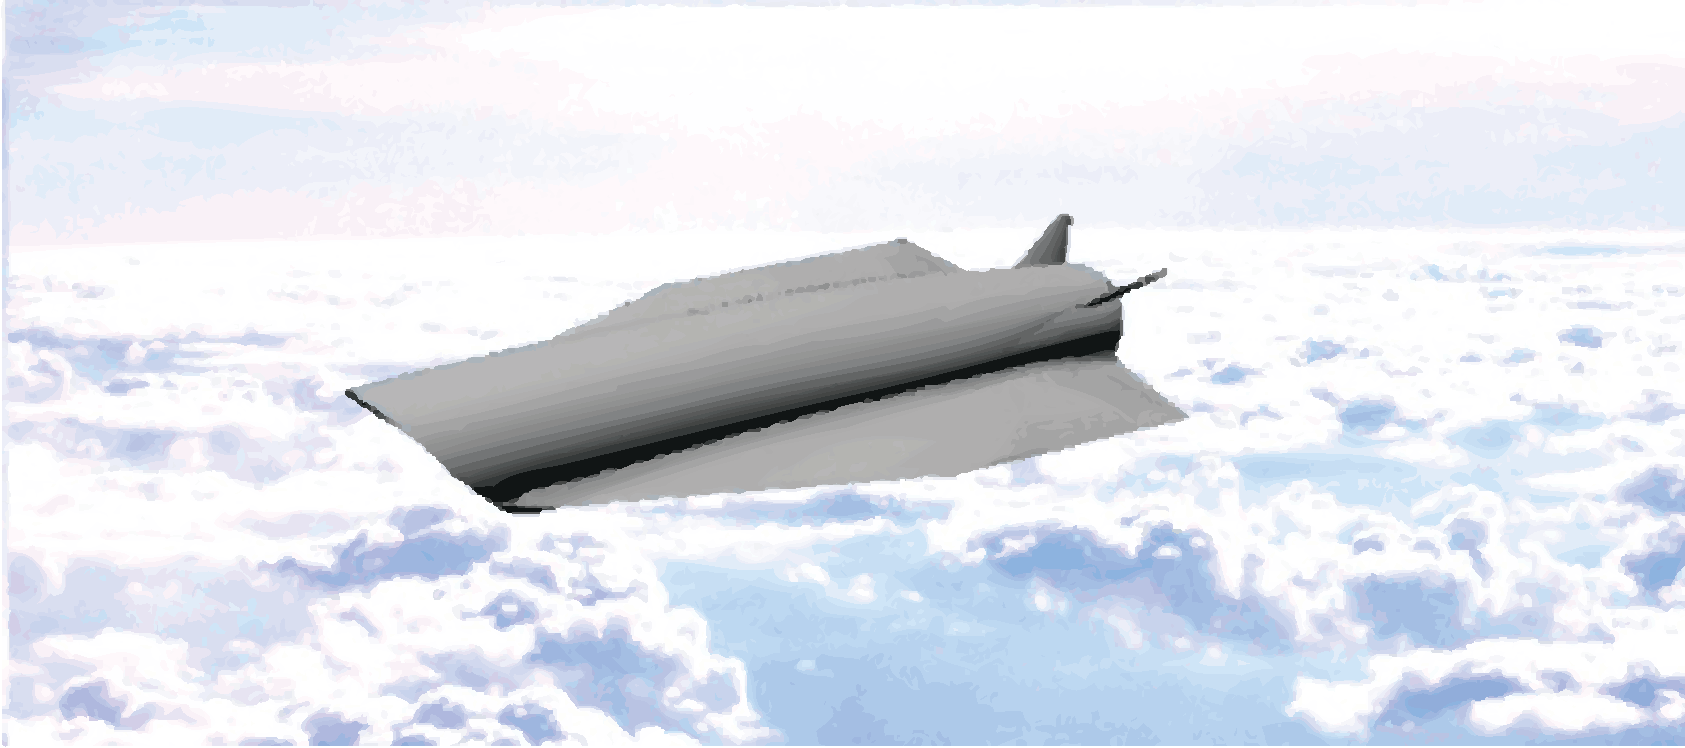
\includegraphics[width=4cm]{\figurepath/ghvclouds.pdf}};
        \node[squareblock, minimum height=1cm, minimum width=2cm, right of=block4,node distance=4.0cm] (block5) {Sensors};
        \node[output, right of=block5,node distance=2.5cm] (output1) {};
        \node[input, below of=block2,node distance=1.5cm](input2){};
        \draw [->]  (b1inA) + (-2.5cm,0cm) -> node [pos=0.15]{$z_{\text{cmd}}$}  (b1inA);
        \draw [->]  (b1inB) + (-0.5cm,0cm) -> (b1inB);
        \draw [->]  (b2inA) + (-1cm,0cm) -> (b2inA);
        \draw [->]  (b2inB) + (-2.0cm,0cm) -> node[name=TB,node distance=2.5cm]{} (b2inB);
        \draw[->](block5) --  node[name=yi,pos=0.4]{}(output1);
        \draw[-](yi) |- (input2);
        \draw[-](b1inB) + (-0.5cm,0cm) -- (2B2);
        \draw[-](b1inA) + (-1.0cm,0cm) -- (2A2) ;
        \draw[-] (b2inB) + (-2.0cm,0cm) |- (input2);
        \draw[->](block1) -- node[pos=0.22]{$u_{\text{bl}}$} node[pos=0.9]{$+$} (sum1);
        \draw[->](block2) -| node[pos=0.1]{$u_{\text{ad}}$} node[pos=0.9]{$+$} (sum1);
        \draw[->](sum1) -- (block3);
        \draw[->](block3) -- (block4);
        \draw[->](block4) -- (block5);
        \begin{pgfonlayer}{background}
          \path (block1 |- block1)+(-2.5,0.7) node (c) {};
          \path (block2 -| block2)+(3.0,-0.7) node (d) {};
          \path[fill=gray!20, draw, dashed] (c) rectangle (d);
        \end{pgfonlayer}
        \node [below of=block2, node distance = 0.9cm] {Controller};
      \end{tikzpicture}
      \caption{Baseline plus adaptive control block diagram \label{fig.baseplusadaptiveblock}}
    \end{center}
  \end{figure}

  Adaptive controllers will be added to the longitudinal and lateral control subsystems.
  Augmenting the uncertain linear plant in Eq.\ \eqref{eqn:xdotpunc} with an integral error state gives the following
  \begin{equation}
    \label{eqn:uncertainss}
    \begin{bmatrix}
      \dot{x}_{p} \\
      \dot{x}_{e}
    \end{bmatrix}=
    \begin{bmatrix}
      A_{p} & 0 \\
      -C_{pz} & 0
    \end{bmatrix}
    \begin{bmatrix}
      x_{p} \\
      x_{e}
    \end{bmatrix}+
    \begin{bmatrix}
      B_{p}\Lambda{W_{p}}^{\top} & 0 \\
      0 & 0
    \end{bmatrix}
    \begin{bmatrix}
      x_{p} \\
      x_{e}
    \end{bmatrix}+
    \begin{bmatrix}
      B_{p} \\
      0
    \end{bmatrix}\Lambda u+
    \begin{bmatrix}
      0 \\
      I
    \end{bmatrix}z_{\text{cmd}}
  \end{equation}
  Equation (\ref{eqn:uncertainss}) can be expressed using $W^{\top}=[\begin{array}{cc} {W_{p}}^{\top} & 0\end{array}]$ as
  \begin{equation*}
    \begin{bmatrix}
      \dot{x}_{p} \\
      \dot{x}_{e}
    \end{bmatrix}=
    \begin{bmatrix}
      A_{p} & 0 \\
      -C_{pz} & 0
    \end{bmatrix}
    \begin{bmatrix}
      x_{p} \\
      x_{e}
    \end{bmatrix}+
    \begin{bmatrix}
      B_{p} \\
      0
    \end{bmatrix}\Lambda W^{\top}
    \begin{bmatrix}
      x_{p} \\
      x_{e}
    \end{bmatrix}+
    \begin{bmatrix}
      B_{p} \\
      0
    \end{bmatrix}\Lambda u+
    \begin{bmatrix}
      0 \\
      I
    \end{bmatrix}z_{\text{cmd}}
  \end{equation*}
  The integral augmented, uncertain plant for which an adaptive controller will be designed is given by
  \begin{equation}
    \label{eqn:uncplant}
    \dot{x}=(A+B\Lambda W^{\top})x+B\Lambda u+B_{\text{ref}}z_{\text{cmd}}
  \end{equation}
  where $A_{\lambda}=A+B\Lambda W^{\top}$.

  \subsection{Classical Model-Reference Adaptive Controller}\label{sec:classicalmrac}

  The reference model for this classical model-reference adaptive controller is selected by apply the nominal full state feedback controller $u_{\text{bl}}=K_{\text{lqr}}^{\top}x$ to the nominal plant model, where $K_{\text{lqr}}$ is the baseline control gain gain that was calculated to optimize control of the nominal plant.
  That is, using the augmented nominal state and input matrices
  \begin{equation*}
    A=
    \begin{bmatrix}
      A_{p} & 0 \\
      -C_{pz} & 0
    \end{bmatrix}
    \quad
    B=
    \begin{bmatrix}
      B_{p} \\
      0
    \end{bmatrix}
    \quad
    B_{m}=B_{\text{ref}}
  \end{equation*}
  with the nominal control gain $K_{\text{lqr}}$, the reference model is given by
  \begin{equation}
    \label{eqn:xodotm}
    \dot{x}_{m}^{o}=A_{m}x_{m}^{o}+B_{m}z_{\text{cmd}}
  \end{equation}
  where $A_{m}=A+BK_{\text{lqr}}^{\top}$ is a Hurwitz matrix.
  This reference model will provide the nominal response which will be used in calculating the tracking error which will drive adaptation.

  With the reference model given in Eq. (\ref{eqn:xodotm}), the tracking error $e^{o}$ is defined as
  \begin{equation}
    \label{eqn:eoerror}
    e^{o}=x-x_{m}^{o}
  \end{equation}
  The adaptive control law is defined as
  \begin{equation}
    \label{eqn:uadporm}
    u_{\text{ad}}=\theta(t)^{\top}x
  \end{equation}
  where $\theta(t) \in \mathbb{R}^{n\times m}$ is the adaptive parameter.
  The following adaptive control gain update law is proposed, where $P^{o}=P^{o\top}>0$, and details on the projection operator are found in references [\citen{lavretskywisebook},\citen{PometPraly.1992}].
  \begin{equation}
    \label{eqn:ormupdatelaw}
    \dot{\tilde{\theta}}=\text{Proj}_{\Gamma}(\theta,-\Gamma^{o} xe^{o\top}P^{o}B\text{sign}(\Lambda))
  \end{equation}
  The total control is given by summing the nominal and adaptive components giving
  \begin{equation}
    \label{eqn:utotal}
    u=(K_{\text{lqr}}+\theta)^{\top}x
  \end{equation}
  Substituting the control law in equation (\ref{eqn:utotal}) into equation (\ref{eqn:uncplant}) the closed-loop system becomes
  \begin{equation*}
    \dot{x}=\left[A+B\Lambda W^{\top}+B\Lambda(\theta+K_{\text{lqr}})^{\top}\right]x+B_{\text{ref}}z_{\text{cmd}}
  \end{equation*}
  Comparing this expression to the reference model, the existence of an ideal feedback gain matrix $\theta^{*}$ that results in perfect reference model tracking can be verified from the following expression.
  \begin{equation}
    \label{eqn:matchingcondition}
    A+B\Lambda W^{\top}+B\Lambda(\theta^{*}+K_{\text{lqr}})^{\top}=A+BK_{\text{lqr}}^{\top}
  \end{equation}
  The adaptive parameter error is defined as
  \begin{equation}
    \tilde{\theta}=\theta-\theta^{*}
  \end{equation}
  Differentiating Eq. (\ref{eqn:eoerror}), and substituting Eq. (\ref{eqn:uncplant}) and (\ref{eqn:xodotm}) in, the error equation can be expressed as
  \begin{equation*}
    \dot{e}^{o}=A_{\lambda}x+B\Lambda u+B_{\text{ref}}z_{\text{cmd}}-[A_{m}x_{m}^{o}+B_{m}z_{\text{cmd}}]
  \end{equation*}
  Substituting Eq. (\ref{eqn:utotal}), and using $B_{m}=B_{\text{ref}}$ the error dynamics become
  \begin{equation*}
    \dot{e}^{o}=Ax+B\Lambda W^{\top}x+B\Lambda(\theta+K_{\text{lqr}})^{\top}x+B_{\text{ref}}z_{\text{cmd}}-A_{m}x_{m}^{o}-B_{\text{ref}}z_{\text{cmd}}
  \end{equation*}
  Using $A_{m}=A+BK_{\text{lqr}}^{\top}$ and Eq. (\ref{eqn:matchingcondition}) the expression
  \begin{equation*}
    A=A_{m}-B\Lambda W^{\top}-B\Lambda(\theta^{*}+K_{\text{lqr}})^{\top}
  \end{equation*}
  is obtained, allowing the error dynamics to be written as
  \begin{equation*}
    \dot{e}^{o}=\left(A_{m}-B\Lambda W^{\top}-B\Lambda(\theta^{*}+K_{\text{lqr}})^{\top}+B\Lambda W^{\top}+B\Lambda(\theta+K_{\text{lqr}})^{\top}\right)x-A_{m}x_{m}^{o}
  \end{equation*}
  which finally simplify to
  \begin{equation}
    \label{eqn:eodotfin}
    \dot{e}^{o}=A_{m}e^{o}+B\Lambda{\tilde{\theta}}^{\top}x
  \end{equation}

  The goal of the adaptive controller is to drive the error $e^{o}(t)$ to zero by adjusting the parameter $\theta(t)$.
  The following candidate Lyapunov equation is proposed, where $\Gamma^{o}\in\mathbb{R}^{n\times n}$ is a symmetric, invertible, positive definite gain matrix, and the operation $|\cdot|$ takes the absolute value of each entry of the matrix argument.

  \begin{equation}
    V(e^{o},\tilde{\theta})=e^{o\top}P^{o}e^{o}+\text{tr}\left(\tilde{\theta}^{\top}\Gamma^{o-1}\tilde{\theta}|\Lambda|\right)
  \end{equation}
  Differentiating
  \begin{equation}
    \label{eqn:Vodot1}
    \dot{V}={\dot{e}}^{o\top}P^{o}e^{o}+e^{o\top}P^{o}\dot{e}^{o}+
    \text{tr}(\dot{\tilde{\theta}}^{\top}\Gamma^{o-1}\tilde{\theta}|\Lambda|)
    +\text{tr}({\tilde{\theta}}^{\top}\Gamma^{o-1}\dot{\tilde{\theta}}|\Lambda|)
  \end{equation}
  Substituting Eq. (\ref{eqn:eodotfin}) into Eq. (\ref{eqn:Vodot1}), and letting $-Q^{o}={A_{m}}^{\top}P^{o}+P^{o}A_{m}$ gives
  \begin{equation}
    \label{eqn:Vodot2}
    \dot{V}=-e^{o\top}Q^{o}e^{o}+2x^{\top}{\tilde{\theta}}\Lambda{B}^{\top}P^{o}e^{o}
    +\text{tr}(\dot{\tilde{\theta}}^{\top}\Gamma^{o-1}\tilde{\theta}|\Lambda|)
    +\text{tr}({\tilde{\theta}}^{\top}\Gamma^{o-1}\dot{\tilde{\theta}}|\Lambda|) \\
  \end{equation}
  Substituting Eq. (\ref{eqn:ormupdatelaw}) into Eq. (\ref{eqn:Vodot2}) and letting $y=-xe^{o\top}P^{o}B\text{sign}(\Lambda)$ gives
  \begin{equation}
    \dot{V}=-e^{o\top}Q^{o}e^{o}
    +2\text{tr}\left(\tilde{\theta}^{\top}\left(\Gamma^{o-1}\text{Proj}_{\Gamma}(\theta,-\Gamma^{o}y)-y\right)|\Lambda|\right)
  \end{equation}
  Using the following property of the projection operator\ \cite{lavretskywisebook}
  \begin{equation}
    \tilde{\theta}^{\top}(\Gamma^{-1}\text{Proj}_{\Gamma}(\theta,\Gamma y)-y)\leq 0
  \end{equation}
  implies $\dot{V}(e^{o},\theta)\leq 0$.
  Thus, the candidate Lyapunov function which was proposed does serve as a valid Lyapunov function for this system.

  \subsection{Closed-Loop Model-Reference Adaptive Controller}\label{sec:crmmrac}

  In this section, a modification to the classical model-reference adaptive controller described in Section~\ref{sec:adaptivedesign}.\ref{sec:classicalmrac} is introduced.
  This modification includes an observer-like gain in the reference model, with feedback from the state $x$.
  This is referred to as a closed-loop reference model (CRM), and can provide improved transient properties over the classical model-reference adaptive controller, which we denote as the open-loop reference model (ORM) controller.\cite{gibson.aiaacrm.2012,gibson.acc1.2013}
  The modified reference model is given by
  \begin{equation}
    \label{eqn:xcdotm}
    \dot{x}_{m}^{c}=A_{m}x_{m}^{c}+B_{m}z_{\text{cmd}}-L(x-x_{m}^{c})
  \end{equation}
  From Eq. (\ref{eqn:xcdotm}) it can be seen that the inclusion of the gain $L$ allows the closed-loop reference model response to deviate from that of the open-loop reference model.
  In the case when the gain $L$ is reduced to zero, the open-loop reference model is recovered.
  The modified reference model Jacobian is defined as
  \begin{equation}
    \label{eqn:ambar}
    \overline{A}_{m}=A_{m}+L
  \end{equation}
  and the tracking error is given by
  \begin{equation}
    \label{eqn:ecerror}
    e^{c}=x-x_{m}^{c}
  \end{equation}
  For the CRM adaptive controller, the same adaptive control law as Eq. (\ref{eqn:uadporm}) is used
  \begin{equation}
    \label{eqn:uadpcrm}
    u_{\text{ad}}=\theta(t)^{\top}x
  \end{equation}
  with the following update law
  \begin{equation}
    \label{eqn:crmupdatelaw}
    \dot{\tilde{\theta}}=\text{Proj}_{\Gamma}(\theta,-\Gamma^{c} xe^{c\top}P^{c}B\text{sign}(\Lambda))
  \end{equation}
  Note that this update law is the same as that in Eq. (\ref{eqn:ormupdatelaw}) used for the ORM adaptive controller, with the exception of the tracking error term $e^{c}$ now being used in the place of $e^{o}$.
  The following candidate Lyapunov function is proposed
  \begin{equation*}
    V(e^{c},\tilde{\theta})=e^{c\top}P^{c}e^{c}+\text{tr}\left(\tilde{\theta}^{\top}\Gamma^{-1}\tilde{\theta}|\Lambda|\right)
  \end{equation*}
  which has time derivative
  \begin{equation*}
    \dot{V}=-e^{c\top}Q^{c}e^{c}
    +2\text{tr}\left(\tilde{\theta}^{\top}\left(\Gamma^{-1}\text{Proj}_{\Gamma}(\theta,-\Gamma y)-y\right)|\Lambda|\right) \\
  \end{equation*}
  As in the ORM case, this implies $\dot{V}(e^{c},\theta)\leq 0$.
  Thus, the candidate Lyapunov function which was proposed serves as a valid Lyapunov function for this system.
  It can also be shown that $e^{c}\rightarrow e^{o}$ as $t\rightarrow\infty$.

  The inclusion of the feedback gain $L$ in the reference model allows the closed-loop reference model response to depart from the open-loop reference model response.
  While this can provide improved transient response\cite{gibson.ecc.2013,gibson.ieeetrans.2013,gibson.acc2.2013} and other benefits which are observed in simulation, there is also the potential for $L$ to be made sufficiently large so as to deteriorate the time response of the system.
  The ideal time response of the system is essentially defined by the open-loop reference model, and the goal is to minimize the tracking error $e^{o}$.
  However, in attempting to realize some benefits through the addition of $L$, the closed-loop reference model behavior will be allowed to deviate from the open-loop reference model.
  In doing so, while the tracking error $e^{c}$ may be very small, the overall time response of the system may be poor due to large differences between the behavior of the two reference models.
  So, while using the error $e^{c}$ to drive adaptation can improve performance, the tracking error $e^{o}$ should still be considered in analyzing performance of the adaptive control system.

  \section{Simulation Results}

  The following figures show the time response of the GHV with the baseline and baseline+adaptive controllers when subjected to parametric uncertainties during a nominal cruise flight condition at $M=6$, $h=80,000$.

  The simulation cases below represent two desired tasks, each with one of three uncertainties.
  The tasks are: $3$ degree angle of attack doublet (1) and $80$ degree roll step (2).
  The uncertainties are: reduction in control effectiveness (A), rearward CG shift (B), $C_{m_{\alpha}}$ scaled (C), and sensor bias on sideslip angle measurement (D).
  Gaussian white noise was introduced into the plant output, and the input delay was set to zero for these simulation results.

  \begin{figure}[H]
    \begin{center}
      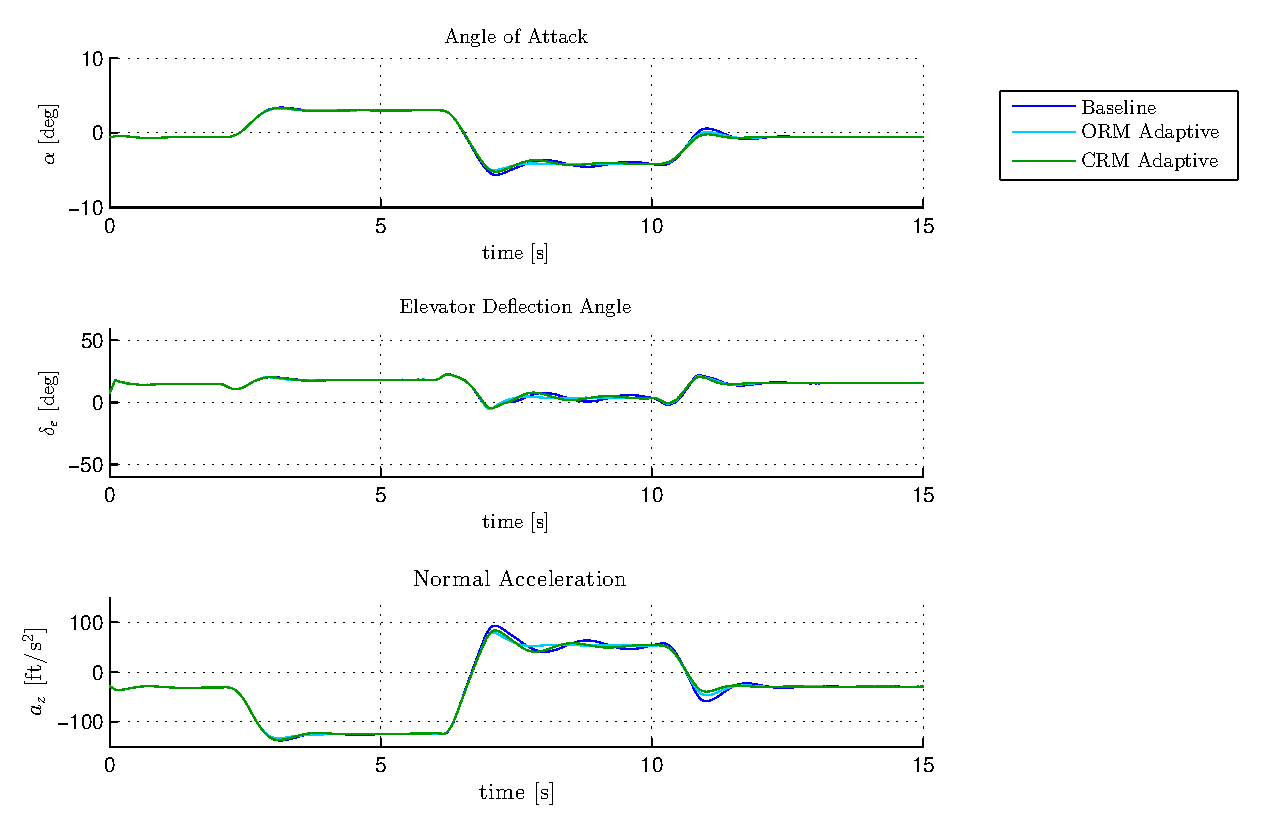
\includegraphics[width=5.0in]{\figurepath/select_longres_cef050b.eps}
      \caption{1A:\ 50\% control surface effectiveness on all surfaces}
    \end{center}
  \end{figure}

  \begin{figure}[H]
    \begin{center}
      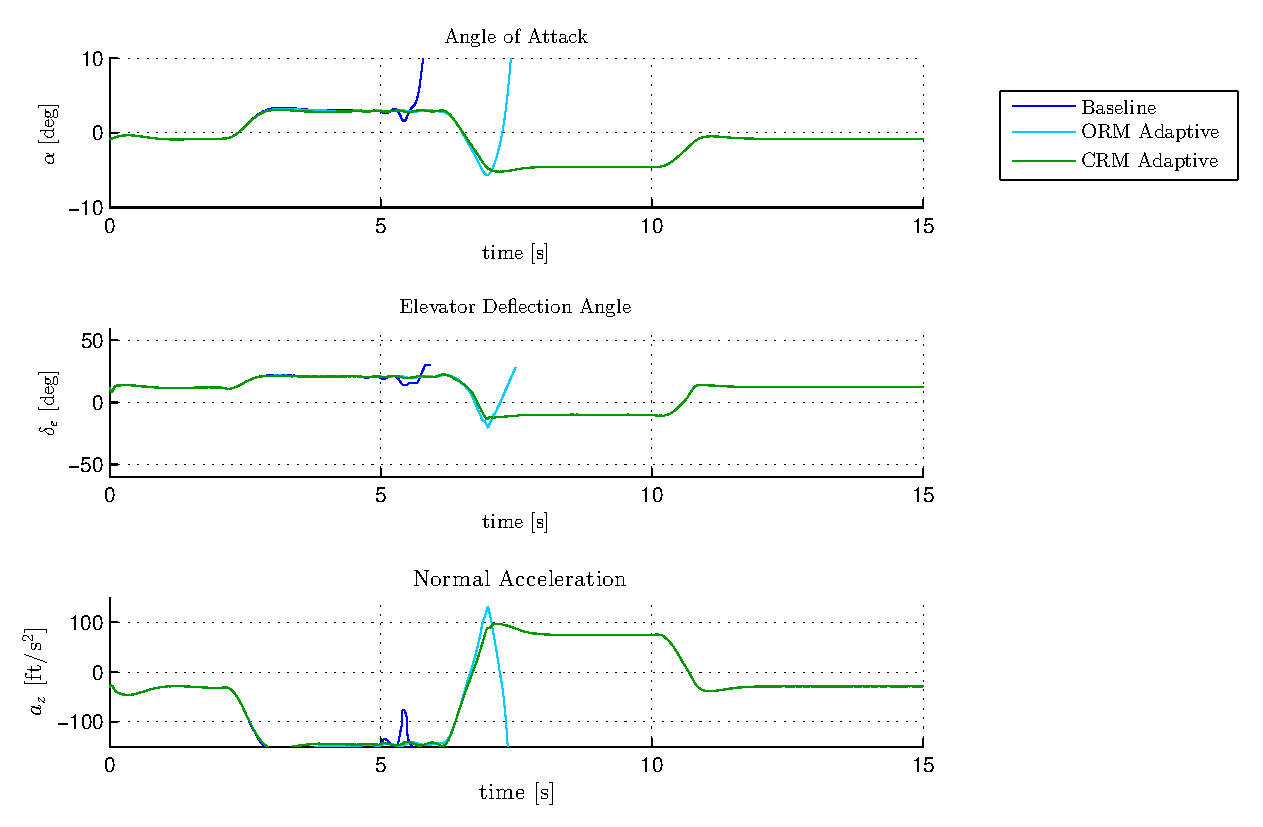
\includegraphics[width=5.0in]{\figurepath/select_longres_cgx090b.eps}
      \caption{1B:\ Longitudinal CG shift: -0.9 ft rearward (6\% of the vehicle length)}
    \end{center}
  \end{figure}

  \begin{figure}[H]
    \begin{center}
      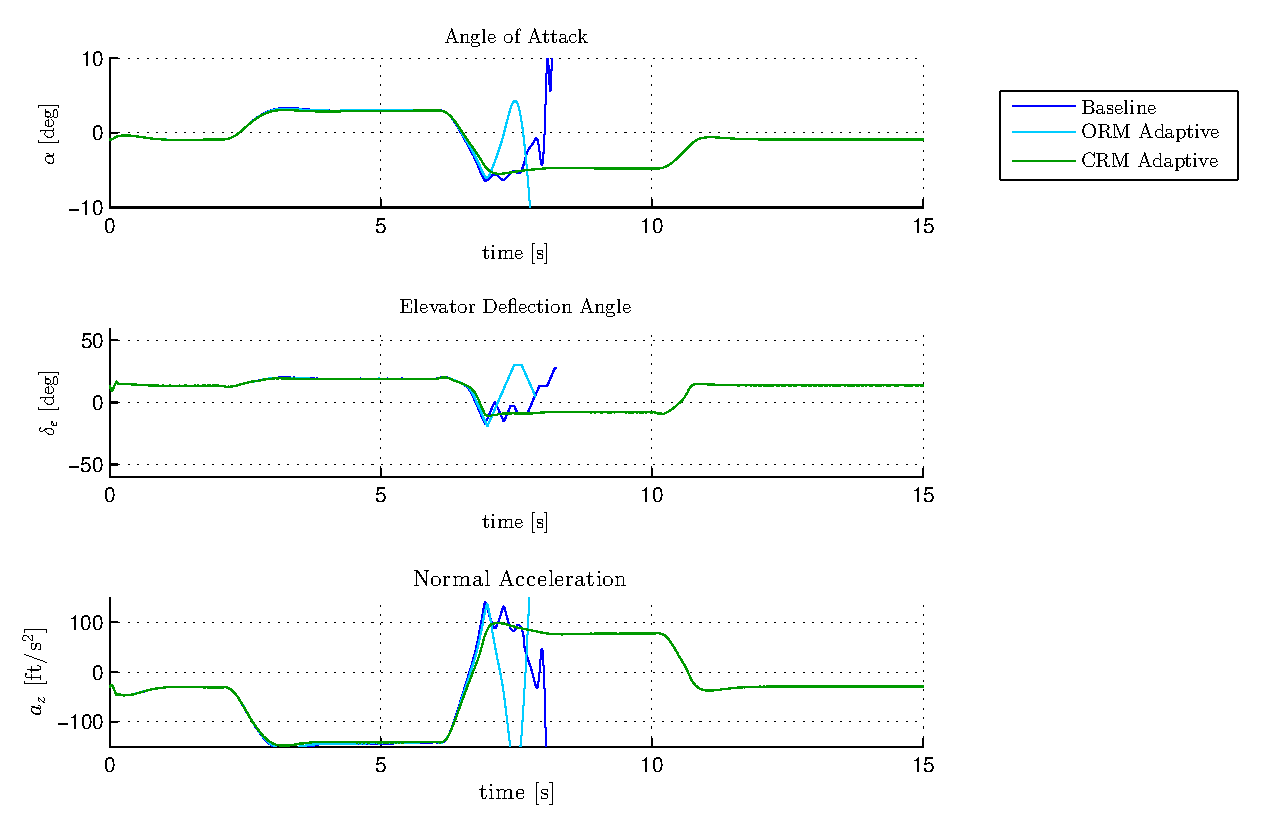
\includegraphics[width=5.0in]{\figurepath/select_longres_cma400b.eps}
      \caption{1C:\ Pitching moment coefficient $C_{m_{\alpha}}$ scaled $4\times$}
    \end{center}
  \end{figure}

  \begin{figure}[H]
    \begin{center}
      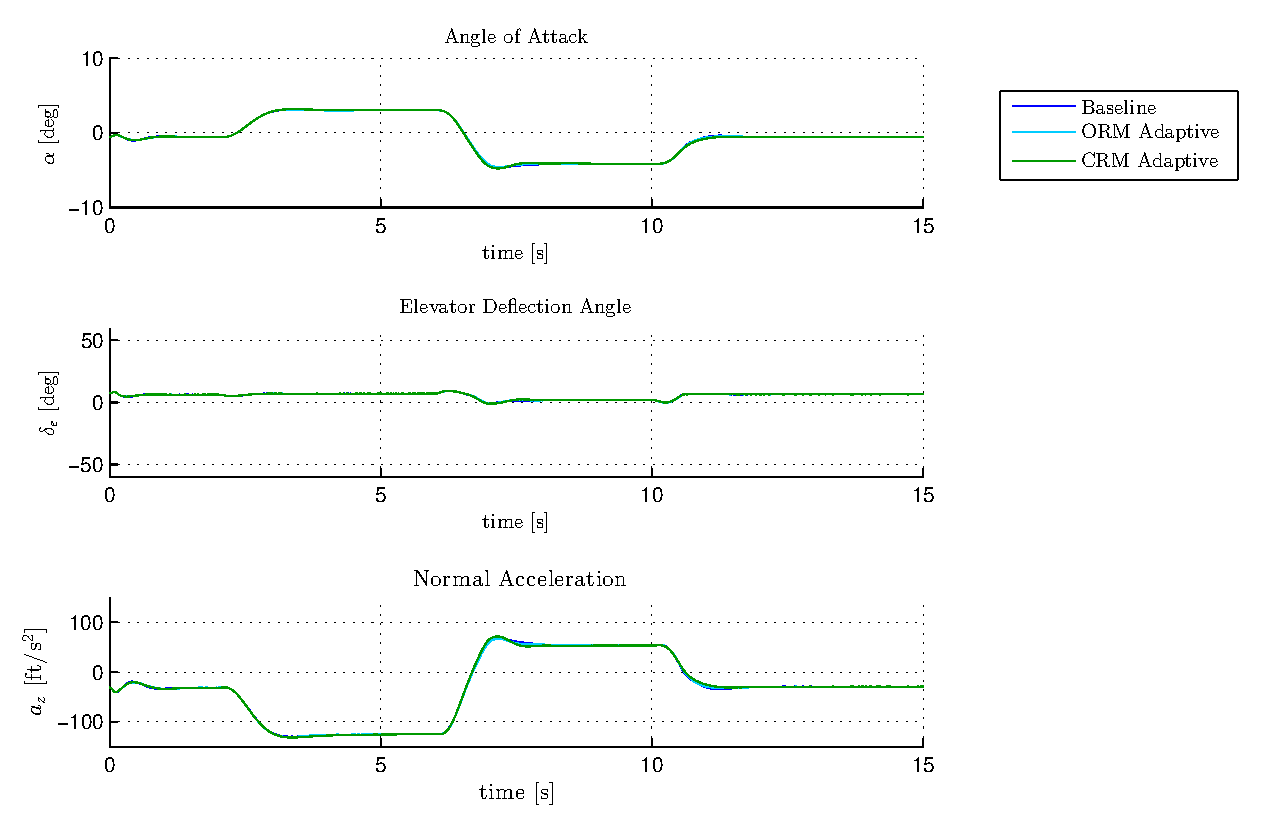
\includegraphics[width=5.0in]{\figurepath/select_longres_bia020c.eps}
      \caption{1D:\ Sensor bias of $+2.0$ degrees on sideslip measurement}
      \vspace{-0.2in}
    \end{center}
  \end{figure}

  \begin{figure}[H]
    \begin{center}
      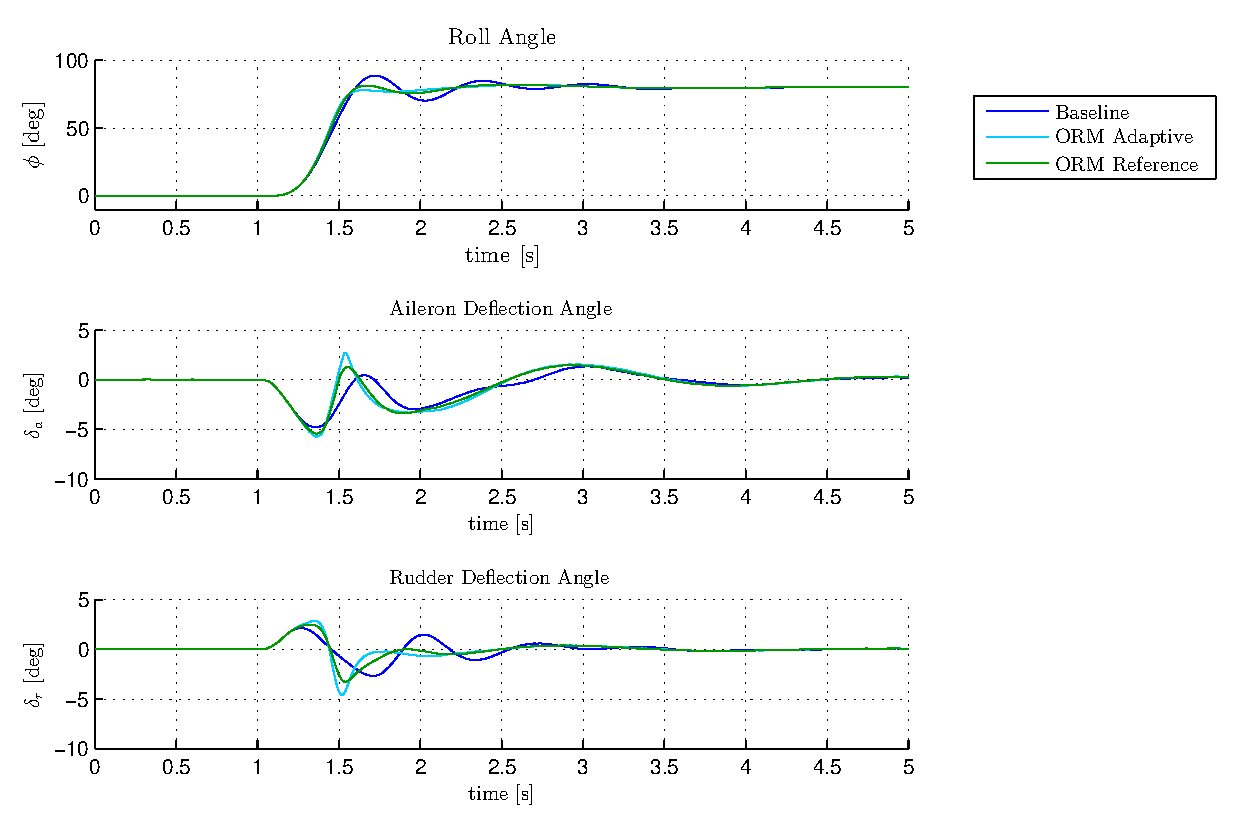
\includegraphics[width=4.9in]{\figurepath/select_latrres_cef050b.eps}
      \caption{2A:\ 50\% control surface effectiveness on all surfaces}
    \end{center}
  \end{figure}

  \begin{figure}[H]
    \begin{center}
      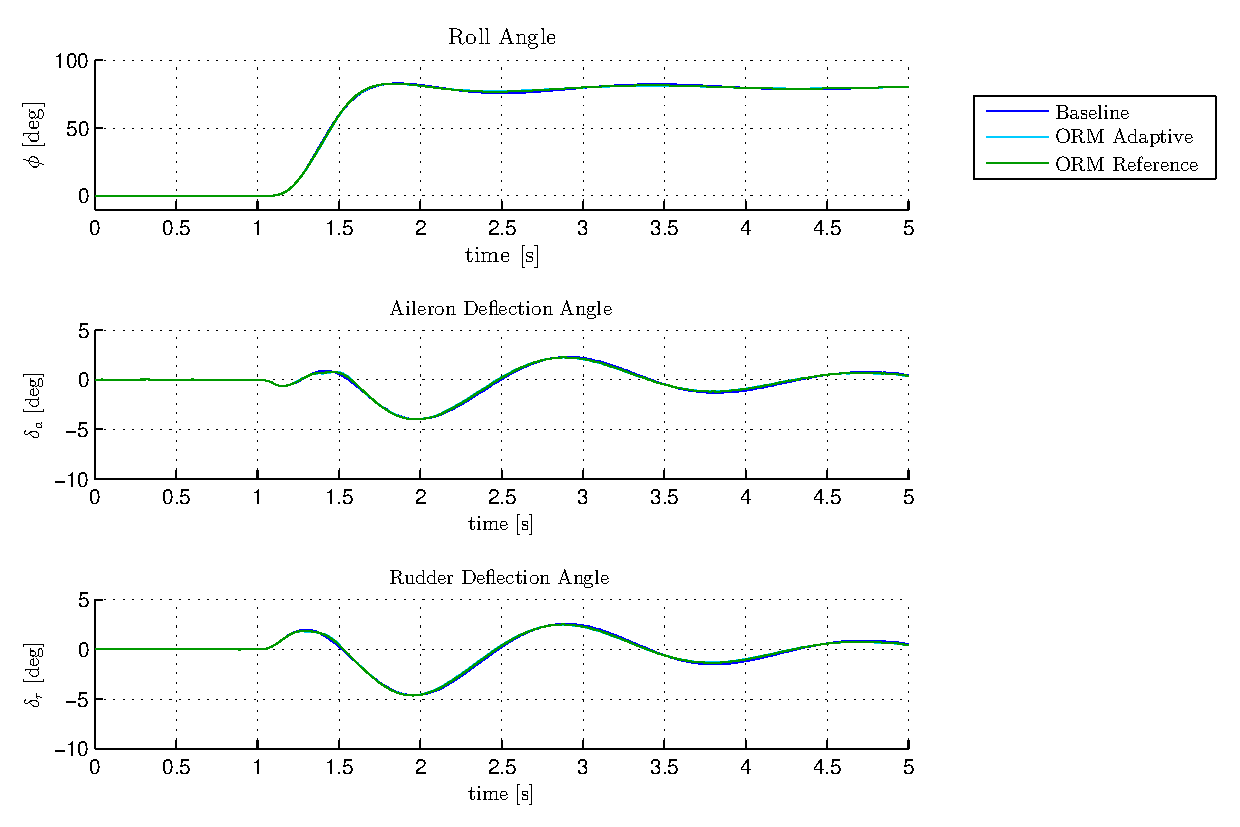
\includegraphics[width=5.0in]{\figurepath/select_latrres_cgx160b.eps}
      \caption{2B:\ Longitudinal CG shift: -1.6 ft rearward (11\% of the vehicle length)}
      \vspace{-0.2in}
    \end{center}
  \end{figure}

  \begin{figure}[H]
    \begin{center}
      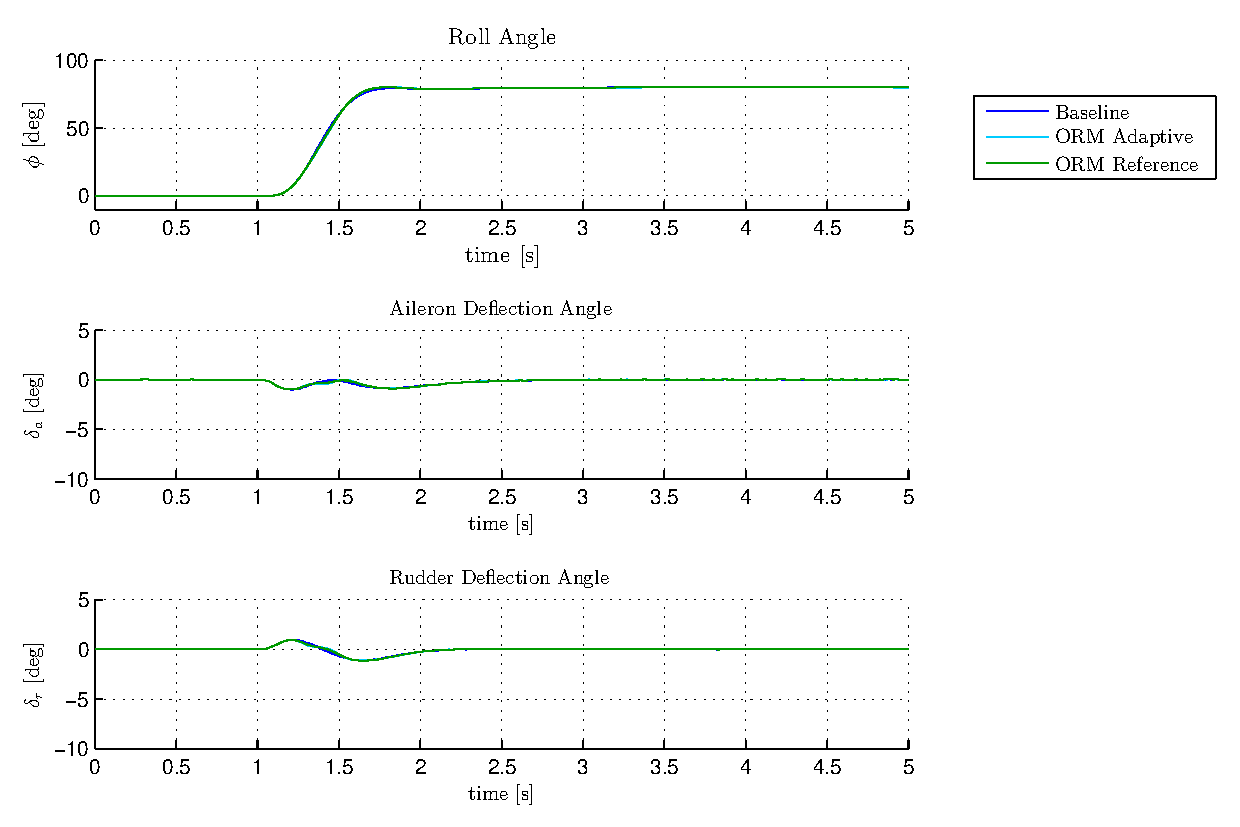
\includegraphics[width=5.0in]{\figurepath/select_latrres_cma400b.eps}
      \caption{2C:\ Pitching moment coefficient $C_{m_{\alpha}}$ scaled $4\times$}
      \vspace{-0.2in}
    \end{center}
  \end{figure}

  \begin{figure}[H]
    \begin{center}
      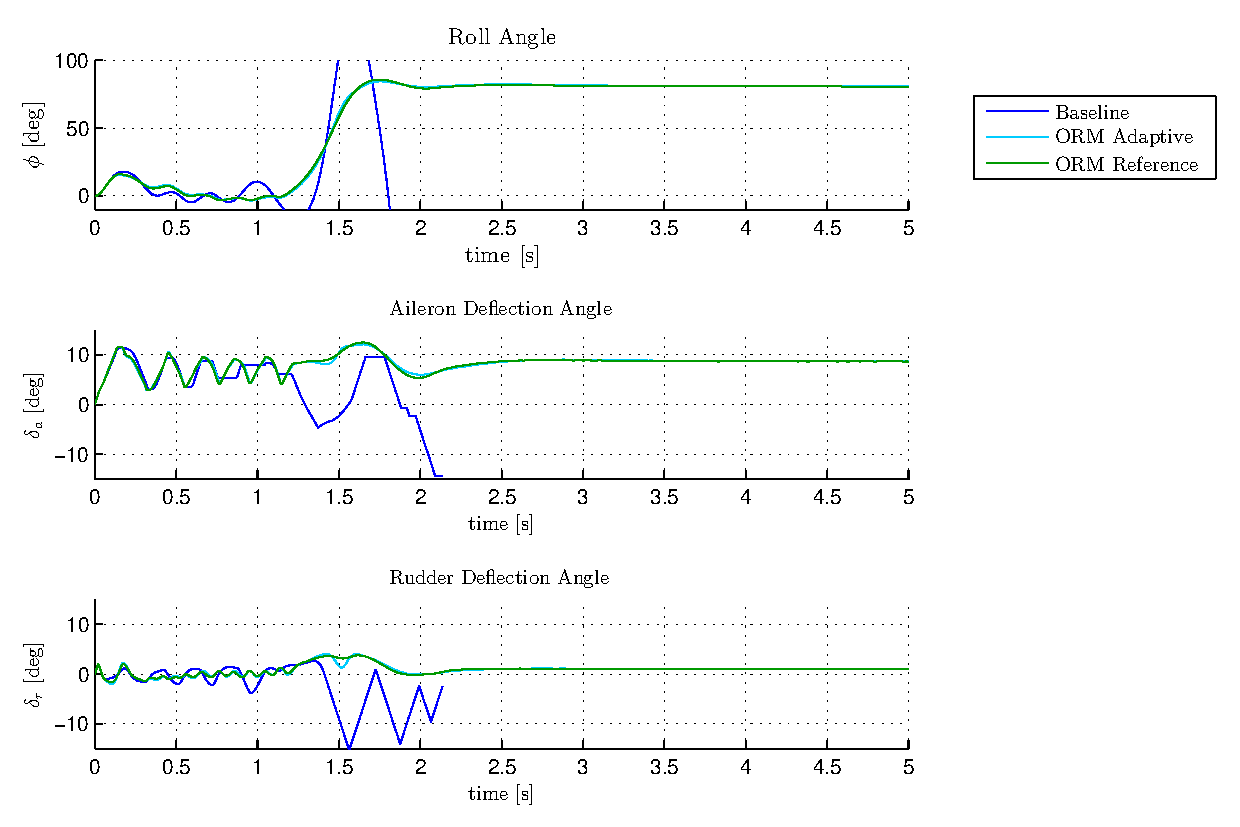
\includegraphics[width=5.0in]{\figurepath/select_latrres_bia032c.eps}
      \caption{2D:\ Sensor bias of $+3.2$ degrees on sideslip measurement}
    \end{center}
  \end{figure}

  In many of the cases presented here, the baseline controller is not able to maintain stability for the given task when subject to uncertainty.
  Moreover, the ORM adaptive controller also is not able to maintain stability responses 1B and 1C, whereas the CRM adaptive controller is able to maintain stability.
  For task 1, the CRM adaptive controller provides good closed-loop performance, with good transient response, minimal overshoot, almost no oscillations.
  In response 1A, the baseline and ORM adaptive controller oscillate slightly more in the time response.
  This behavior is even more pronounced as control effectiveness is reduced further, to the point where there is insufficient control authority to maintain stability.
  In response 1B, the baseline and ORM adaptive controllers fail to maintain stability.
  This is triggered by an oscillation in the lateral-directional dynamics.
  However, the CRM adaptive controller maintains stability and good time response performance.
  A similar situation is observed in response 1C, as the increased pitching moment coefficient has a very similar influence on the plant dynamics as a rearward CG shift.
  In response 1D, both adaptive controllers perform nearly identically to the baseline controller.

  Response 2A shows the baseline controller again exhibiting significant oscillations in the time response when control effectiveness is reduced.
  Both adaptive controllers significantly reduce this oscillation.
  Minimal benefit of the adaptive controllers is observed in responses 2B and 2C, but this is largely due to the limited affect the longitudinal CG shift and pitching moment coefficient have on the lateral directional dynamics which are excited during the roll command.
  Finally, response 2D shows the baseline controller failing to maintain stability when subject to the sensor bias on the sideslip angle measurement.

  Typically, both the ORM and CRM adaptive controllers have similar performance in terms of rise time and settling time, with the CRM controller typically requiring slightly decreased control effort.
  Both adaptive controllers have more highly damped response when compared to the baseline controller, thus better tracking the desired command.
  Overall, both adaptive controllers show improved performance over the baseline controller in every case.

  \subsection{Time Delay Margins}

  For each of the tasks and uncertainties demonstrated in simulation above, time delay margins were computed empirically for the three controllers by determining the maximum allowable input time delay that could be tolerated while maintaining stability.
  Table~\ref{tab:delaymargins} shows the delay margins for each case, with varying values of the uncertainties.

  \begin{table}[H]
    \centering
    \caption{Delay margins (ms)\label{tab:delaymargins}}
    \small
    \begin{tabular}{llrrr}
      \toprule
      & & \multicolumn{3}{c}{Controller} \\
      Task & Uncertainty & Baseline & ORM & CRM \\
      \midrule
      \multirow{5}{*}{1} & none & 34 & 38 & 38 \\
      & A:\ 50\% & 33 & 36 & 41 \\
      & B:\ -0.6 ft & 10 & 13 & 15 \\
      & C:\ 3.5$\times$ & 8 & 1 & 15 \\
      & D:\ $+$2.0 deg & 23 & 16 & 17 \\
      \midrule
      \multirow{5}{*}{2} & none & 40 & 24 & 28 \\
      & A:\ 50\% & 34 & 13 & 26 \\
      & B:\ -1.6 ft & 24 & 18 & 20 \\
      & C:\ 3.5$\times$ & 22 & 19 & 21 \\
      & D:\ $+$2.0 deg & 23 & 18 & 20 \\
      \bottomrule
    \end{tabular}
  \end{table}

  In most of the cases shown here, the ORM adaptive controller deteriorates some of the delay margin provided by the baseline controller.
  However, in every case the CRM adaptive controller has a delay margin equal to, or greater than the ORM controller.
  The delay margin of the CRM controller is at least 70\% that of the baseline controller, while the ORM controller has a delay margin which is as little as 13\% of that for the baseline controller.
  Adaptation is required to maintain stability and provide good tracking performance, but must do so without sacrificing the delay margin to an unacceptable level.
  The CRM adaptive controller is able to satisfy these requirements better than both the baseline and ORM adaptive controllers.

  \section{Conclusion}

  The performance of a generic hypersonic vehicle was evaluated during angle of attack and roll commands, when subject to a loss of control effectiveness, stability derivative uncertainties, longitudinal CG shift, and sensor bias, while in the presence of sensor noise, and input delay.
  Three controllers were considered: a baseline full-state feedback LQR-PI, and the same baseline controller augmented with a classical open-loop reference model adaptive controller, as well as a closed-loop reference model adaptive controller.
  Both adaptive controllers exhibited improved performance and stability over the baseline controller when given a commanded trajectory in the presence of parametric uncertainties.

  In three of the simulation cases shown, the baseline controller was not able to maintain stability.
  The ORM adaptive maintained stability in all but two cases, and the CRM adaptive controller maintained stability in all cases.
  In addition, considering the cases where stable performance was maintained by both the baseline and adaptive controllers, the CRM adaptive showed improved time response behavior over the other two controllers.
  Finally, when a time delay was introduced at the control input, the CRM adaptive controller maintained a greater percentage of the time-delay margin provided by the baseline controller than the ORM adaptive controller did.
  Overall, the CRM adaptive controller offers the best performance, tolerating a reduced control effectiveness of 50\%, rearward center of gravity shift of -0.9 to -1.6 feet (6--11\% of vehicle length), aerodynamic coefficient uncertainty scaled $4\times$ the nominal value, and sensor bias of up to $+3.2$ degrees on sideslip angle measurement.
  The closed-loop reference model adaptive controller maintains at least 70\% of the delay margin provided by the robust baseline design, tolerating input time delays of at least 15 ms during 3 degree angle of attack doublet, and 80 degree roll step commands.
  These results demonstrate the necessity of an adaptive controller to provide stable and acceptable tracking performance, while still maintaining much of the delay margin provided by the robust baseline design.

  \section{Acknowledgment}

  Approved for Public Release; Distribution Unlimited.
  Case Number 88ABW--2013--3392.

  \bibliography{\bibsourcepath}
  \bibliographystyle{../sty/aiaa}
\end{document}
